\documentclass{article}
\usepackage{amstext}
\usepackage[
    web={centertitlepage,designv,forcolorpaper,tight*,latextoc,extended},
    eforms={usealtadobe,setcorder},aebxmp
]{aeb_pro}
%\usepackage[ImplMulti]{dljslib}
\usepackage{graphicx,array,fancyvrb}
\usepackage{aeb_mlink}
%\usepackage{myriadpro}
%\usepackage{calibri}
\usepackage[altbullet]{lucidbry}

\usepackage{xbmks}
\DeclareInitView{layoutmag={navitab:UseOutlines}}
\xbmksetup{colors={int=red},styles={intbf}}


\makeatletter
\renewcommand*\l@section[2]{%
  \ifnum \c@tocdepth >\z@
    \addpenalty\@secpenalty
    \addvspace{.75em \@plus\p@}% make less space
    \setlength\@tempdima{1.5em}%
    \begingroup
      \parindent \z@ \rightskip \@pnumwidth
      \parfillskip -\@pnumwidth
      \leavevmode \bfseries
      \advance\leftskip\@tempdima
      \hskip -\leftskip
      #1\nobreak\hfil \nobreak\hb@xt@\@pnumwidth{\hss #2}\par
    \endgroup
  \fi}
\makeatother

\let\tops\texorpdfstring

\def\FmtMP#1{\marginpar{\small\itshape\raggedleft#1}}

\hfuzz2pt
%\makePDasXOn

%\previewOn\pmpvOn

\def\hardspace{{\fontfamily{cmtt}\selectfont\symbol{32}}}
\let\uif\textsf

\advance\marginparwidth12pt

\usepackage{acroman}
\usepackage[active]{srcltx}

\edef\amtIndent{\the\parindent}

\addtolength{\marginparwidth}{2pt}

\urlstyle{tt}

\def\STRUT{\rule{0pt}{14pt}}

\makeatletter
\newcount\hesheCnt \hesheCnt=-1
\def\heshe{\@ifstar{\heshei}{\global\advance\hesheCnt1\relax\heshei}}
\def\heshei{\ifodd\hesheCnt she\else he\fi}
\def\HeShe{\@ifstar{\HeShei}{\global\advance\hesheCnt1\relax\HeShei}}
\def\HeShei{\ifodd\hesheCnt She\else He\fi}
\def\hisher{\@ifstar{\hisheri}{\global\advance\hesheCnt1\relax\hisheri}}
\def\hisheri{\ifodd\hesheCnt her\else his\fi}
\def\himher{\@ifstar{\himheri}{\global\advance\hesheCnt1\relax\himheri}}
\def\himheri{\ifodd\hesheCnt her\else him\fi}
\makeatother

\DeclareDocInfo
{
    university={\AcroTeX.Net},
    title={The \textsf{thorshammer} Package},
    author={D. P. Story},
    email={dpstory@acrotex.net},
    subject=Documentation for the thorshammer package,
    talksite={\url{www.acrotex.net}},
    version={1.5.11, 2021/06/24},
    Keywords={assessment workflow, LaTeX, AcroTeX},
    copyrightStatus=True,
    copyrightNotice={Copyright (C) \the\year, D. P. Story},
    copyrightInfoURL={http://www.acrotex.net}
}

\universityLayout{fontsize=Large}
\titleLayout{fontsize=LARGE}
\authorLayout{fontsize=Large}
\tocLayout{fontsize=Large,color=aeb}
\sectionLayout{indent=-62.5pt,fontsize=large,color=aeb}
\subsectionLayout{indent=-31.25pt,color=aeb}
\subsubsectionLayout{indent=0pt,color=aeb}
\subsubDefaultDing{\tops{$\bullet$}{\textrm\textbullet}}


\chngDocObjectTo{\newDO}{doc}
\begin{docassembly}
var titleOfManual="The thorshammer Package";
var manualfilename="Manual_BG_Print_thorshammer.pdf";
var manualtemplate="Manual_BG_Brown.pdf"; // Blue, Green, Brown
var _pathToBlank="C:/Users/Public/Documents/ManualBGs/"+manualtemplate;
var doc;
var buildIt=false;
if ( buildIt ) {
  console.println("Creating new " + manualfilename + " file.");
  doc = \appopenDoc({cPath: _pathToBlank, bHidden: true});
  var _path=this.path;
  var pos=_path.lastIndexOf("/");
  _path=_path.substring(0,pos)+"/"+manualfilename;
  \docSaveAs\newDO ({ cPath: _path });
  doc.closeDoc();
  doc = \appopenDoc({cPath: manualfilename, oDoc:this, bHidden: true});
  f=doc.getField("ManualTitle");
  f.value=titleOfManual;
  doc.flattenPages();
  \docSaveAs\newDO({ cPath: manualfilename });
  doc.closeDoc();
} else {
    console.println("Using the current "+manualfilename+" file.");
}
var _path=this.path;
var pos=_path.lastIndexOf("/");
_path=_path.substring(0,pos)+"/"+manualfilename;
\addWatermarkFromFile({
    bOnTop:false,
    bOnPrint:false,
    cDIPath:_path
});
\executeSave();
\end{docassembly}

\begin{document}

\maketitle

\pdfbookmarkx[1]{Title Page}[action={\Named{FirstPage}}]{TitlePage}
\pdfbookmarkx[1]{Documentation of the system scripts}[action={\GoToR/F(thmclass.pdf)/D[0 /Fit]},color=blue,style={bf}]{sysscripts}
\pdfbookmarkx[1]{How to install Action sequences}[action={\GoToR/F(install-action-seq.pdf)/D[0 /Fit]},color=blue,style={bf}]{instAS}
\pdfbookmarkx[1]{Links to AcroTeX.Net}[action={/S/GoTo/D(undefined)},%
  color=magenta,style={bf}]{acrotex}
\belowpdfbookmarkx{http://www.acrotex.net}[action={\URI{http://www.acrotex.net}},%
  color=magenta,style={bf}]{home}
\belowpdfbookmarkx{http://blog.acrotex.net}[action={\URI{http://blog.acrotex.net}},%
  color=magenta,style={bf}]{blog}


\selectColors{linkColor=black}
\tableofcontents
\selectColors{linkColor=webgreen}

\section{Acknowledgements}

The author would like to acknowledge Thorsten G. (a.k.a., Thor) who proposed
this workflow and who contributed many ideas, the proposed workflow I found
to be interesting and worth my time developing the idea; and to J\"{u}rgen G.
(a.k.a., Loki) who also contributed many good ideas, enthusiasm, questions,
bug detection, and motivation. High regards and respect to both.
\begin{flushright}
D. P. Story (a.k.a., Odon)
\end{flushright}

\begin{center}
  \fbox{%
    \parbox{.75\linewidth}{\textbf{\textcolor{red}{Warning!}} The workflow of the \pkg{thorshammer}
    package requires the instructor to use \textbf{\textsf{Adobe Acrobat
    XI}}, or later. Any PDF creator may be used to build the quizzes,
    however, but \app{Acrobat} is needed to execute one-time JavaScript
    (\cs{sadQuizzes}) and to run the action sequences (formerly called batch
    sequence by \app{Adobe}) such as \textsf{Thor's way}. Only \app{Adobe
    Reader} is required for the students. Of course, this is the
    full-featured \app{Adobe Reader} of a desktop or laptop, not the
    \app{Adobe Reader} found on tablets, smartphones, and such.
  }}%
\end{center}

\section{Introduction}\label{intro}

Thor has asked me to assist him in creating a quiz system, based on
Acro\negthinspace\TeX, to be delivered to his classes. His workflow for this
assessment system is as follows:\footnote{As my occasional friend J\"{u}rgen
says, this workflow is a real hammer, so I titled this package `Thors(ten)
hammer', or simply \pkg{thorshammer}.}
\begin{enumerate}
   \item The \env{quiz} environment is used to pose the questions, which
      consist of MC, numerical fill-in the blank, and \emph{extended response
      questions}.\footnote{Extended response questions are the interesting
      part.} Though the \env{quiz} environment is used, the score is not
      reported to the student upon finishing the quiz.
   \item The students takes the quiz in a computer lab, each student has
       {\hisher} own personal student folder. The quizzes are dropped into the
       personal folders.
   \item When the student finishes the exam, taken in \app{AR},\footnote{\app{AR}
       refers to \app{Adobe Reader DC}.} {\heshe} presses the \textsf{End
       Quiz} control and saves the document.
   \item At some point, the instructor's script moves the student quizzes
       to the instructor's folder.
   \item The instructor opens the PDF and finishes marking the extended
       response questions and assigns a grade.
   \item System scripts then returns the quizzes to the students.
\end{enumerate}
The original concept was expanded considerably as the package was developed:
extensive \hyperref[s:sysscrpts]{system scripts} were written to support the
system; and \hyperref[actSeq]{action sequences} were written, also to support
Thor's way.


\section{Preliminaries}

Most important is the correct installation of \pkg{thorshammer} along with
its required packages and folder JavaScript files. These are discussed in
this section.

\subsection{Package requirements}

The most recent version of the packages \pkg{insdljs} (2021/06/19),
\pkg{exerquiz} (2021/05/29), \pkg{eq-save} (2021/04/27) are required. These
three packages were modified slightly to obtain features needed by
\pkg{thorshammer}.

The \pkg{thorshammer} package requires the folder JavaScript files
\texttt{aeb\_pro.js}\FmtMP{\textsf{aeb\_pro.js}} (Version 1.6.2 or later,
required) and \texttt{aeb-reader.js}\FmtMP{\textsf{aeb-reader.js}} (Version
1.0 or later); these two are distributed by the
\pkg{acrotex-js}\FmtMP{\pkg{acrotex-js} pkg} package, dated 2021/06/24 or
later, and are found in \texttt{js-files} folder
of the distribution of \pkg{acrotex-js}. These files give access to
security restricted JavaScript methods. If you already have \pkg{aeb\_pro}
installed, be sure you have Version 1.6.2 of \texttt{aeb\_pro.js}, if not,
install Version 1.6.2 provided by the \pkg{acrotex-js} distribution.

The \texttt{aeb\_pro.js} is used on the instructor's system, along with
\app{Acrobat} (\app{AA}), to author quizzes. \app{Distiller} is not used
unless the author prefers a TEX $\rightarrow$ DVI $\rightarrow$ PS
$\rightarrow$ PDF workflow, using \app{Distiller} as the PDF creator. For
this workflow, \app{pdflatex}, \app{lualatex}, and \app{xelatex} will work as
PDF creators; however, \app{Acrobat} is needed to execute the JavaScript code
generated by the command \cs{sadQuizzes} and to execute the action sequences
provided by this package.

Once the quizzes are created, the author can take the quizzes in \app{Adobe
Reader} (\app{AR}) to get the same experience as his students. Additionally,
\texttt{aeb-reader.js}\FmtMP{\textsf{aeb-reader.js}} can be installed on the
student's work environment, if possible/permitted; \texttt{aeb-reader.js}
contains a subset of JavaScript methods taken from \texttt{aeb\_pro.js} that
\emph{will enhance student experience}. The author can install this file on
his system to take the quizzes in the same environment, again using
\app{Adobe Reader}. \textbf{Warning:}\FmtMP{\textbf{Warning}} Do not install
\texttt{aeb\_pro.js} in any folder where an \app{Adobe Reader} is used by
students.

\paragraph*{Other enhancements to user experience.} \app{Adobe Reader} is by default in \uif{Protected Mode}.
When \uif{Protected Mode} is enabled, one or more security dialog boxes popup
as the student saves his/her document. To eliminate this annoyance, clear the
\uif{Enable Protected Mode at startup} checkbox, as shown in the
\hyperref[fig:PM]{Figure~\ref*{fig:PM}}. On your personal system, open
\app{AR}, press \uif{Ctrl+K}\FmtMP{\uif{Ctrl+K}}, select \uif{Security
(Enhanced)} from the \uif{Categories} panel, finally, clear the checkbox, as
shown in \hyperref[fig:PM]{Figure~\ref*{fig:PM}}.\footnote{For \app{AA}, this
checkbox is cleared by default.} The installation of \texttt{aeb-reader.js}
and clearing the checkbox to disable \uif{Protected Mode} most likely require
the sysadmin\FmtMP{sysadmin permission} to make those changes.
\begin{figure}[htb]\centering
\includegraphics[width=\linewidth]{graphics/protected-mode}
\caption{Clear \textsf{Protected Mode} checkbox}\label{fig:PM}
\end{figure}

%which gives access to security restricted JavaScript methods used by this
%package.\footnote{If you have the \pkg{aeb\_pro} package already installed,
%the you also have \texttt{aeb\_pro.js} (Version 1.7.2 or later, required);
%you can use \texttt{aeb\_pro.js} instead of \texttt{aeb-reader.js}.}
%Additionally, the file \texttt{aeb\_pro.js}\FmtMP{\textsf{aeb\_pro.js}} is
%required to be correctly installed on your computer. The file comes with the
%\pkg{aeb\_pro} package, though the package itself is not required. As a convenience,
%\texttt{aeb\_pro.js} is also include in the \texttt{folder-js} folder.

\paragraph*{Installation of JS files for \app{Acrobat}.} The description of the installation of
the JavaScript file \texttt{aeb\_pro.js} is provided by the \pkg{acrotex-js}
package; read the \texttt{install\_jsfiles.pdf} file found in the
\texttt{docs} folder of the \pkg{acrotex-js} package.

\paragraph*{Installation of JS files for \app{Adobe Reader}.} The folder JavaScript
file \texttt{aeb-reader.js} may be installed for use by \app{Adobe Reader} as
well. Installing \texttt{aeb-reader.js} enhances the experience of the
students as they save their quiz document after completing the quiz.
Normally, it is not possible to install such a JavaScript file for use by
students; however, if the students take the quiz in a Computer Lab, the
sysadmin\FmtMP{sysadmin} can install \texttt{aeb-reader.js} on all the computers used in the
Computer Lab.  Discussion of how and where to install folder JavaScript files
is found in the file \texttt{docs/install\_jsfiles.pdf} of the
\pkg{acrotex-js} package. Read and follow the directions carefully.
(\app{Reader} looks for its folder JavaScript files in the same location
where \app{Acrobat} would look for them.)


\subsection{Package options}

There are seven options for this package.
\begin{description}
 \item[\opt{nocfg}] There is a language localization file, discussed in
     Section~\ref{s:lang}, that is loaded as a matter of course. When this
     option is taken, the configuration file is not loaded. In this case,
     the default English language definitions are used for all strings.
 \item[\opt{testmode}] When this option is specified, the quizzes are
     regular quizzes that can be tested in the usual \pkg{exerquiz}-way. A
     \textsf{Correct} button is available to correct the quiz.
 \item[\opt{!testmode}] A convenience option for putting the document into
     the default mode: Quizzes are ready to be taken by the students,
     pressing the \textsf{End Quiz} does not give any score for their
     effort, but students are prompted to save the quiz.
 \item[\opt{useclass}] Use this option to bring in additional code to
     declare each member of the class, to automatically build a custom quiz
     for each class member, to distribute these quizzes to a designated
     folder of the instructor, and to distribute the quizzes the respective
     class folder. Refer to Section~\ref{ss:uc} for details.
  \item[\opt{usebatch}] This option executes the \opt{useclass} option;
      however, there is a batch sequence, called \textsf{Thor's way}, that
      the instructor uses to process all class quizzes after the class has
      finished with them. Refer to Section~\ref{ss:ub} for details.
  \item[\opt{batchdistr}] The option automatically passes the
      \opt{usebatch} and the \opt{useclass} options.
      Additionally, the document assembly script does not
      distribute copies of the quizzes to the student folders,
      rather, it is expected the author uses either
      \textsf{Thor distributes} or \textsf{Thor protects and
      distributes} action wizards to perform the distribution
      task. The quizzes can later be distributed using an
      operating system script. Refer to Section~\ref{ss:bd}
      for details.
 \item[\opt{ordinary}] When this option is passed, ordinary
     quizzes are created, \emph{ones that do not follow Thor's
     Hammer workflow}. The \opt{testmode} option is
     automatically executed, as well as other changes. Refer
     to section~\ref{ordinary} for more details and examples.
\end{description}

\section{Necessary conditions that would make this system work}

In recent years, browser technology has \emph{devolved} to the point that
\app{Adobe Reader} is no longer supported---with the exception of Microsoft's
\app{Internet Explorer~11}---within a browser window. For documents using
\pkg{exerquiz}, which relies heavily on \app{Acrobat} JavaScript API,
interactive quizzes can no longer be taken within a brower; hence, if an
instructor wants to use \pkg{exerquiz} to author quizzes to be taken by
{\hisher} students, the quizzes must be taken on a desktop or laptop from
within the \app{Adobe Reader} application.\footnote{At this time, \app{Adobe
Reader} on mobile and tablets do not support form fields and JavaScript.}

\subsection{The effectiveness of using PDF quizzes for assessment}

The effectiveness of an in-class quiz is closely tied to quiz security. In a
normal classroom setting, students take the quiz/test---all at the same
time---under the glaring gaze of responsible adult. This is to ensure there
is no `cheating.' This is the method used for paper quizzes/tests that are a
major part of the students grade. However, security becomes more lax when
students work on assignments with lesser weight in the final grade. Homework
assignments are an example.

For PDF quizzes, the philosophy is the same, for lesser credit, the students
can take the quizzes on their own. If the quizzes are for major credit in the
course, then one would expect stricter security.

\paragraph*{The ideal condition.} The following list comprises the ideal conditions
for assessment using PDF quizzes.
\begin{itemize}
  \item \textbf{An exam period.} There is a definite (time) period the
      students are to take the quizzes. The quizzes are moved to the
      private student folders at the beginning of the assessment period,
      and removed again at the end of the assessment.
  \item  The ideal condition is for the students to take the quiz only in a
      CBT lab (computer-based testing lab) under supervision.

  \item \textbf{CBT Lab.} The student must use \app{Adobe Reader}, must not
      use email or a thumb-drive (to transmit the PDF quiz), and must not
      print the quiz. For Thor's workflow, the student finds the quiz in
      the his/her personal folder.

  \item \textbf{No access to private folder.} The students do not have access to the private folder outside of
      the CBT lab.
\end{itemize}
The workflows devised in this package will work well for class quizzes taken under these ideal conditions.

\subsection{Authoring a quiz}

The \pkg{thorshammer} package uses post-pdf creation JavaScript methods. For
these methods to have any effect, the document author must use the \app{Adobe
Acrobat}\FmtMP{\app{Acrobat} required} application. The PDF creation can be
any of the usual {\LaTeX} workflows: \app{dvips/Adobe Distiller},
\app{pdflatex}, \app{lualatex}, or \app{xelatex}. In all cases, after PDF
creation, the newly created file must be opened in \app{Acrobat} before any
auxiliary files are deleted. When opened in \app{Acrobat} the first time,
certain code lines of JavaScript execute to perform a number of tasks.

There is another JS file that needs to be either located or created, the file
name is \texttt{config.js}\FmtMP{edit \textsf{config.js}}. It is a standard
\app{Acrobat} file and is located in the same folder in which
\texttt{aeb-reader.js} (or, perhaps, \texttt{aeb\_pro.js}) reside. The file
\texttt{install\_jsfiles.pdf}, found in the \texttt{docs} folder, discusses
where \app{Acrobat} expects to find folder JavaScript files. Find or create
\texttt{config.js} and insert the following line:
\begin{Verbatim}[xleftmargin=\amtIndent,commandchars=!~@]
var _thorshammer=true;!quad//!sffamily~ secret variable@
\end{Verbatim}
This JavaScript variable plays an interesting role: Certain form elements in
the quiz only appear when this variable is present, in particular, the
\textsf{Mark it} control only appears when the document is opened in
\app{Acrobat} and the above script line appears in the \texttt{config.js}
file.\footnote{\textbf{Important!} Do not install \texttt{config.js} where
any \app{AR} used by a student; otherwise, the \textsf{Mark It} control will
be displayed to the student, which we don't want.} You'll have to see it to
believe it.

\newtopic\noindent
Once the quiz has been built, the quizzes themselves require only \app{Adobe
Reader} to take.

\newpage

\section{Workflows for interactive assessment using PDF}

The document author has several choices for student/instructor experience. We
discuss these in this section.

\subsection{Basic methods}\label{ss:BMs}

A \emph{basic method}\FmtMP{basic method} is one in which none of the ``class options'' are used; these
are \opt{useclass}, \opt{usebatch}, and \opt{batchdistr}.
This method is illustrated in sample file \texttt{thexb.tex}. Compiling this file
produces a single quiz, which is distributed to the class.

\subsubsection{Preamble}

\begin{Verbatim}[xleftmargin=\amtIndent,fontsize=\small,commandchars={!~@}]
\documentclass{article}
\usepackage{amstext}              %!textsf~ (optional, used in a minor way below)@
\usepackage{web}                  %!textsf~ (optional)@
\usepackage[usealtadobe]{insdljs}
\usepackage[usesumrytbls]{exerquiz}
!textbf~\usepackage{thorshammer}@          %!textsf~ (basic methods imply no options taken)@

\setInitMag{fitwidth}                %!textsf~ (optional, defined in this package)@
\hypersetup{pdfpagelayout=OneColumn} %!textsf~ (optional, from hyperref )@

%!textsf~ Optional customizations@
%\useNameToCustomize
%\enumQuizzes{3}
%\instrPath{/C/Users/!ameta~username@/Desktop/Test Folder/target/_Thor}
%\classPath{/C/Users/!ameta~username@/Desktop/Test Folder/target/myClass}
%\distrQuizzes{{A/_Thor}{B/_Thor}{C/_Thor}}

\reversemarginpar
\showCreditMarkup  %!textsf~ always include this command, it is required@
%\previewOn\pmpvOn
\useBeginQuizButton[\CA{Begin}]
\useEndQuizButton[\CA{End}]
\PTsHook{($\eqPTs^{\text{pts}}$)}
\useMCCircles

%!textsf~ Declare the quiz name@
\DeclareQuiz{q1}
%!textsf~ Post document creation JavaScript@
\begin{docassembly}
\sadQuizzes
\end{docassembly}
\begin{document}
...
\end{Verbatim}
There are two new commands and one new environment above to mention:
\bVerb\small\takeMeasure{\string\setInitMag\darg{fitpage|actualsize|fitwidth|fitheight|fitvisible|inheritzoom}}%
\begin{dCmd}[fontsize=\small]{\bxSize}
\setInitMag{fitpage|actualsize|fitwidth|fitheight|fitvisible|inheritzoom}
\end{dCmd}
\eVerb This command determines the initial magnification. There are a choice
of six values for the argument; the default is \texttt{fitpage}.

\paragraph*{Optional customizations.}\label{para:OCs} There are a several commands to customize the creation of
the quizzes.
\bVerb\small\takeMeasure{\string\distrQuizzes\darg{\darg{*\ameta{path\SUB1}}\darg{*\ameta{path\SUB2}}...\darg{*\ameta{path\SUB{num}}}}}%
\begin{dCmd}[fontsize=\small,commandchars=!()]{\bxSize}
\useNameToCustomize
\enumQuizzes{!ameta(num)}
\instrPath{!ameta(path)}
\classPath{!ameta(path)}
\distrQuizzes{{*!ameta(path!SUB1)}{*!ameta(path!SUB2)}...{*!ameta(path!SUB(num))}}
\end{dCmd}
\eVerb When none of these commands appear in the preamble, compiling the quiz
document, produces a single quiz; e.g., compiling \texttt{thexb.tex} produces
\texttt{thexb.pdf}. Otherwise, compiling \texttt{thexb.tex} produces, for
example, enumerated copies of the quiz files:
\texttt{thexb-1.pdf}, \texttt{thexb-2.pdf}, \dots,
\texttt{thexb-\meta{num}.pdf}.
\begin{description}
    \item[\cs{useNameToCustomize}] When the instructor makes the final
        assessment, {\heshe} presses the \textsf{Mark It} button and a
        \textsf{Save As} dialog box opens: by default, the name of the
        current file is pre-filled into the \textsf{File name} input field;
        if \cs{useNameToCustomize} is in force, however, when \textsf{Mark
        It} is pressed, the suggested file name in the \textsf{Save As}
        dialog box is pre-filled as
        \texttt{\cs{jobname}-\ameta{first}\_\ameta{last}-g.pdf}, where
        \cs{jobname} is the base name of the original {\LaTeX} source file.
        The values of \ameta{first} and \ameta{last} are taken from the
        name fields of the document, where the student is expected to enter
        {\hisher} name.
    \item[\cs{enumQuizzes\darg{\ameta{num}}}] When this command is present
        in the preamble, the command \cs{sadQuizzes} (described below)
        creates \ameta{num} copies of the quiz, and labels them
        \cs{jobname-1.pdf}, \cs{jobname-2.pdf}, \dots,
        \cs{jobname-\meta{num}.pdf}.
    \item [\cs{instrPath\darg{\ameta{path}}}] (The instructor folder) The
        \cs{instrPath} command is the path to the folder of the instructor.
        A copy of all quizzes produced are placed at the end of this path.
    \item [\cs{classPath\darg{\ameta{path}}}] (The class folder root) The
        \cs{classPath} command is the path to the root of the class folders
        of the students.
    \item[\cs{distrQuizzes\darg{*\darg{\ameta{path\SUB1}}\darg{*\ameta{path\SUB2}}...\darg{*\ameta{path\SUB{num}}}}}]
        The argument takes a series of paths: (1) if the star-option
        (\texttt*) is \emph{not present}, then \ameta{path} is the relative
        path to the student folder, relative to the class folder root; (2)
        if the star-option (\texttt*) is present, the \ameta{path} is the
        full path to the student folder. Each folder path is enclosed in
        braces (\darg{}).
\begin{Verbatim}[fontsize=\small]
\classPath{/C/Users/dpstory/Desktop/Test Folder/target/myClass}
\newcommand{\altClassPath}
  {/C/Users/dpstory/Desktop/Test Folder/target/myOtherClass}
\distrQuizzes{{A/_Thor}{*\altClassPath/B/_Thor}{C/_Thor}}
\end{Verbatim}
Quizzes are placed (by \cs{sadQuizzes}) in the student folders:
\begin{Verbatim}[fontsize=\small]
/C/Users/dpstory/Desktop/Test Folder/target/myClass/A/_Thor}
/C/Users/dpstory/Desktop/Test Folder/target/myOtherClass/B/_Thor}
/C/Users/dpstory/Desktop/Test Folder/target/myClass/C/_Thor}
\end{Verbatim}
When the \cs{classPath}/\cs{distrQuizzes} combination is used, the
\cs{enumQuizzes} command is ignored. The number of quizzes to be created is
determined by the number of folder paths listed in \cs{distrQuizzes}.
\end{description}

\paragraph*{Declaring quiz name.} Also in preamble is the declaration of the quiz name.
\begin{Verbatim}[xleftmargin=\amtIndent,commandchars={!~@}]
\DeclareQuiz{!ameta~qz-name@}!quad%!textsf~ defined in exerquiz@
\end{Verbatim}
The \ameta{qz-name} should consist of alpha-numeric characters only (eg,
\texttt{quiz1}), and no umlauts, Loki!\footnote{I am informed by the mighty
Thor himself that umlauts can simply rendered in German with `ue' instead of
\"{u}, `oe' instead of \"{o}, and so on; however, we don't want to encourage
Loki. I wish he would have told Loki years ago, it would have saved me a lot
of headaches.} The command saves the quiz name in several ways:
\begin{itemize}
    \item As equivalent text macros, \cs{thisQuiz} and \cs{currQuiz}. Either of these
    of these two must be used to reference the quiz name when you set up the \env{quiz}
    environment; for example,
\begin{Verbatim}[fontsize=\small,commandchars={!~@}]
\DeclareQuiz{q1}
...
\begin{document}
...
\begin{quiz*}{\thisQuiz}!quad%!textsf~ or @\begin{quiz*}{\currQuiz}
...
\end{quiz}
\end{Verbatim}
    \item As the text macro \cs{thQuizName}\FmtMP{\cs{thQuizName}}. This
        command was created to solve a problem with the Thor's hammer. (Can
        you believe it?)  When a parent file has multiple renditions of the
        quiz, Thor's hammer names them differently. For example, if we
        declare \cs{DeclareQuiz\darg{q1}}, in the first rendition, the quiz
        name is \texttt{q1a}, in the second rendition, the quiz name is
        \texttt{q1b}, and so on. (There is a limitation of 26 renditions,
        though the use of alphabetic letters can easily be changed to
        numbers.) The command \cs{thQuizName} always expands the original
        quiz name.
\end{itemize}
While on the topic of quiz names, Thor has forged with his mighty hammer, a
convenience command,
\bVerb\small\takeMeasure{\string\thQzName\darg{\ameta{text}}}%
\setlength{\eflength}{\widthof{\sffamily(\cs{thQuizName})}}%
\edef\x{\the\eflength}%
\setlength{\eflength}{\bxSize}%
\def\1{\rlap{\hskip\eflength\rlap{\hskip\x\relax\qquad\cs{def}\cs{thqzname\darg{\ameta{text}}}}\sffamily(\cs{theQuizName})}}
\begin{dCmd}[fontsize=\small,commandchars=!()]{\bxSize}
!1\thQzName{!ameta(text)}
\end{dCmd}
\eVerb The expression in the parentheses above is the default value; in the third column is the underlying
text macro definition. Declaring \cs{theQzName\darg{Quiz \#1}} defines the text macro \cs{thqzname} that
expands to `Quiz \#1'.

\paragraph*{Post document creation JavaScript.} It is important to insert the \cs{sadQuizzes}
command just above \verb~\begin{document}~, within the \env{docassembly}
environment.
\bVerb\takeMeasure{\string\begin\darg{docassembly}}\par\vskip3pt %\vskip-\baselineskip
\begin{dCmd}[commandchars=!~@]{\bxSize}
\begin{docassembly}
!textbf~\sadQuizzes@
\end{docassembly}
\end{dCmd}
\eVerb The \env{docassembly} environment (also available in the
\pkg{aeb\_pro} package) is a verbatim write environment; it writes its
contents verbatim to the file \texttt{docassembly.cut} then inputs it back in
immediately. In this application, place \cs{sadQuizzes} in the body of the
environment.

\paragraph*{What does \cs{sadQuizzes} do?} The command expands to a series of
JavaScript lines. What is does depends on several factors.
\begin{itemize}
  \item The script identifies the solution pages, extracts and saves them
      to the current folder under the name
      \cs{jobname-thsolns4-\ameta{qz-name}.pdf}; it then removes the
      solution pages from the parent document. The solution pages are later
      appended to the quiz after the students take the quiz by the instructor
      when {\heshe} presses the \textsf{Freeze Quiz} button.
  \item If \cs{enumQuizzes\darg{\ameta{num}}} is used, \cs{sadQuizzes} makes
      \meta{num} copies of the quiz, labeling them \cs{jobname-1.pdf},
      \cs{jobname-2.pdf}, and so on. Files are saved to the folder of the
      source file.
  \item If the \cs{classPath}/\cs{distrQuizzes} combination is used, \cs{sadQuizzes} makes enumerated
  copies of the quiz and places each in a separate folder designated by the argument
  of \cs{distrQuizzes}.
\end{itemize}

\subsubsection{The body of the document}

%The first item in the body is the declaration of the quiz name.
%\begin{Verbatim}[xleftmargin=\amtIndent,commandchars={!~@}]
%\DeclareQuiz{!ameta~qz-name@}!quad%!textsf~ defined in exerquiz@
%\end{Verbatim}
%The \ameta{qz-name} should consist of alpha-numeric characters only (eg,
%\texttt{quiz1}), and no umlauts, Loki!\footnote{I am informed by the mighty
%Thor himself that umlauts can simply rendered in German with `ue' instead of
%\"{u}, `oe' instead of \"{o}, and so on; however, we don't want to encourage
%Loki. I wish he would have told Loki years ago, it would have saved me a lot
%of headaches.} The command saves the quiz name in several ways:
%\begin{itemize}
%    \item As equivalent text macros, \cs{thisQuiz} and \cs{currQuiz}. Either of these
%    of these two must be used to reference the quiz name when you set up the \env{quiz}
%    environment; for example,
%\begin{Verbatim}[fontsize=\small,commandchars={!~@}]
%\DeclareQuiz{q1}
%...
%\begin{document}
%...
%\begin{quiz*}{\thisQuiz}!quad%!textsf~ or @\begin{quiz*}{\currQuiz}
%...
%\end{quiz}
%\end{Verbatim}
%    \item As the text macro \cs{thQuizName}\FmtMP{\cs{thQuizName}}. This
%        command was created to solve a problem with the Thor's hammer. (Can
%        you believe it?)  When a parent file has multiple renditions of the
%        quiz, Thor's hammer names them differently. For example, if we
%        declare \cs{DeclareQuiz\darg{q1}}, in the first rendition, the quiz
%        name is \texttt{q1a}, in the second rendition, the quiz name is
%        \texttt{q1b}, and so on. (There is a limitation of 26 renditions,
%        though the use of alphabetic letters can easily be changed to
%        numbers.) The command \cs{thQuizName} always expands the original
%        quiz name.
%\end{itemize}
%While on the topic of quiz names, Thor has forged with his mighty hammer, a
%convenience command,
%\bVerb\small\takeMeasure{\string\thQzName\darg{\ameta{text}}}%
%\setlength{\eflength}{\widthof{\sffamily(\cs{thQuizName})}}%
%\edef\x{\the\eflength}%
%\setlength{\eflength}{\bxSize}%
%\def\1{\rlap{\hskip\eflength\rlap{\hskip\x\relax\qquad\cs{def}\cs{thqzname\darg{\ameta{text}}}}\sffamily(\cs{theQuizName})}}
%\begin{dCmd}[fontsize=\small,commandchars=!()]{\bxSize}
%!1\thQzName{!ameta(text)}
%\end{dCmd}
%\eVerb The expression in the parentheses above is the default value; in the third column is the underlying
%text macro definition. Declaring \cs{theQzName\darg{Quiz \#1}} defines the text macro \cs{thqzname} that
%expands to `Quiz \#1'.


\newtopic\noindent
Thor \emph{requires}\FmtMP{required} a first and last name field.
\bVerb\takeMeasure{\string\FirstName[\ameta{opts}]\darg{\ameta{wd}}\darg{\ameta{ht}}}%
\begin{dCmd}[commandchars=!()]{\bxSize}
\FirstName[!ameta(opts)]{!ameta(wd)}{!ameta(ht)}
\LastName[!ameta(opts)]{!ameta(wd)}{!ameta(ht)}
\end{dCmd}
\eVerb The \ameta{opts} argument is for changing the appearance of these text
fields. These fields are placed at the top of the quiz.
\bVerb\takeMeasure{\string\thfullnameFmt\darg{\ameta{how-to-format}}}%
\setlength{\eflength}{\bxSize}%
\def\1{\rlap{\hskip\eflength\textsf{(See \texttt{examples/misc/thexrt.tex})}}}
\def\2{\rlap{\hskip\eflength\textsf{(Default: \texttt{\string\thfullnameFmt\darg{\#1+" "+\#2}})}}}
\begin{dCmd}[commandchars=!()]{\bxSize}
!1\FullName[!ameta(opts)]{!ameta(wd)}{!ameta(ht)}
!2\thfullnameFmt{!ameta(how-to-format)}
\end{dCmd}
\eVerb The \cs{FirstName} and \cs{LastName} fields are required; however, the
\cs{FullName} command can explicitly appear as well, perhaps on the cover
page. This command gets its value from the values of the \cs{FirstName} and
\cs{LastName} fields; \ameta{how-to-format} is a JavaScript string that
displays how you want the full name to appear. Within the argument of
\cs{thfullnameFmt}, \texttt{\#1} is the first name and \texttt{\#2} is the
second name. Another example of this formatting is
\verb~\thfullnameFmt{#2+", "+#1}~, here, the full name is presented as last name first, followed by a
command, then the first name. These ideas are demonstrated in
\texttt{examples/misc/thexrt.tex}.

\newtopic
The name fields\FmtMP{importance of the \emph{required} name fields} play a
critical role in Thor's way of doing things. In addition to providing text
fields for the student to identify \himher self, the \emph{required} name
fields are used to mark the beginning of a quiz page. \emph{The required name
fields must appear at the top of the page} and above the beginning of the
quiz. Some of the JavaScript of \pkg{thorshammer} interprets the page on
which the required name fields appear as the page that marks the beginning of
the quiz.

\newtopic\noindent
The following fields are an integral part of Thor's way:
\bVerb\takeMeasure{\string\displaySumryTbl[\ameta{opts}]\darg{\string\currQuiz}}%
\begin{dCmd}[commandchars=!()]{\bxSize}
\markQz[!ameta(opts)]{!ameta(wd)}{!ameta(ht)}
\freezeOrSave[!ameta(opts)]{!ameta(wd)}{!ameta(ht)}
\studentReport[!ameta(opts)]{!ameta(wd)}{!ameta(ht)}
\studentGrade[!ameta(opts)]{!ameta(wd)}{!ameta(ht)}
\begin{sumryTblAux}{\currQuiz}
\displaySumryTbl[!ameta(opts)]{\currQuiz}
\end{sumryTblAux}
\end{dCmd}
\eVerb These commands and environments are aesthetically arranged at the top of the quiz file along with
the name fields, though the \cs{displaySumryTbl} can be placed anywhere (see the \pkg{exequiz} documentation
on this summary table structure).
\begin{description}
\item[\cs{markQz}] This button appears in \app{Acrobat} only when the
    secret variable is detected. After the students have taken the quiz and
    they are back in the possession of the instructor, the instructor opens
    each completed quiz and presses this button, whose default caption is
    \textsf{Mark It}. The underlying script marks up the quiz, showing
    which problems were answered correctly, how many points received for
    each response, etc.

    One of the features of Thor's way is to have extended response
    questions. The student responses to this type of question must be read and
    corresponding points must be assigned in the box provided.
\item[\cs{freezeOrSave}] This button appears only after the \textsf{Mark It} button has been pressed.
  It has two different forms:
  \begin{enumerate}
    \item When the \opt{usebatch} option (or higher) is \emph{not in
        effect}, this button appears with caption \textsf{Freeze Quiz}.
        The action of this button is to attach any solution pages and
        make all form fields \emph{in the entire document} readonly. It
        also flattens all annotations in the document. \emph{Press this
        button only} after all markups are finished and document is ready
        to be moved into the student's folder.

        \item[] \textbf{Control of flattening.} There are options to have the
        \textsf{Freeze Quiz} button to flatten or not.
\cs{thQuizHeader} and \cs{thQuizHeaderLayout}:
\bVerb\takeMeasure{\string\flattenOn\quad\string\flattenOff}%
\begin{dCmd}[commandchars=!()]{\bxSize}
\flattenOn!quad\flattenOff
\end{dCmd}
\eVerb For basic methods, the default is \cs{flattenOff}, while for
  \opt{useclass} it is \cs{flattenOn}. Normally, when you use the
  \opt{useclass} option, all fields are flattened when the \textsf{Freeze
  Quiz} button is pressed. This means you cannot run the quizzes through
  \textsf{Thor's way} to extract the grades; recording of grades is done
  in the tradional way, by hand. However, turning \cs{flattenOff} enables
  you to use \texttt{Thor's way} even with the \opt{useclass} option. (Or,
  simple change the option to \opt{usebatch}.)

        \item[] \textbf{Applies to basic methods.} The following command is
        obeyed only when there is no ``class option'' option specified.
\bVerb\takeMeasure{\string\useNameToCustomize}%
\setlength{\eflength}{\bxSize}%
\def\1{\rlap{\hskip\eflength\sffamily{\enspace Obeyed for basic methods only}}}%
\begin{dCmd}[commandchars=!()]{\bxSize}
!1\useNameToCustomize
\end{dCmd}
\eVerb When the \cs{freezeorSave} button is pressed, the \textsf{Save As}
        dialog is opened to save the file, the file name offered is
        either \cs{jobname.pdf} (the default) or
        \cs{jobname-\ameta{first}\_\ameta{last}-g.pdf} (provided
        \cs{useNameToCustomize} has been expanded in the preamble.
    \item When the \opt{usebatch} option (or higher) option \emph{is in
        effect}, the caption is \textsf{Save \& Close}. As the caption
        suggests, the action is to save the document the current folder
        and close the document in \app{Acrobat}. With the \opt{usebatch}
        option, the implication is that the instructor is to use one of
        the action-wizards to continue processing the students' quizzes.
    \end{enumerate}
\item[\cs{studentReport}] (text field) This readonly field shows the number
    of points awarded and the total points (eg, 15 / 20). The field is initially hidden,
    and becomes visible when \textsf{Mark It} is pressed.
\item[\cs{studentGrade}] (text field) A field for assigning some sort of
    grade, which can be a letter or number. The field is initially hidden,
    and becomes visible when \textsf{Mark It} is pressed.
\end{description}
Speaking of aesthetically pleasing arrangement, \pkg{thorshammer} defines,
\cs{thQuizHeader} and \cs{thQuizHeaderLayout}:
\bVerb\takeMeasure{\string\thQuizHeaderLayout}%
\begin{dCmd}[commandchars=!()]{\bxSize}
\thQuizHeader*
\thQuizHeaderLayout
\end{dCmd}
\eVerb The \cs{thQuizHeader} command does nothing more than to test for the presence of
the \texttt{*} option; if \emph{not present}, a \cs{newpage} command is
issued, otherwise, no \cs{newpage} is forced. Throughout the sample files,
\cs{thQuizHeader} is used. The \cs{thQuizHeaderLayout} is the command that
actually contains the arrangement of the design elements. Do not redefine
\cs{thQuizHeader}; but you may define \cs{thQuizHeaderLayout}; look at
\pkg{thorshammer.dtx} for the definition \cs{thQuizHeaderLayout}, this will
give you  insight for any redefinition.

\paragraph*{Placement.} \cs{DeclareQuiz} is preferably placed in the preamble\FmtMP{preamble} and
\cs{thQuizHeader} is placed prior to the first quiz.
\begin{Verbatim}[xleftmargin=\amtIndent,commandchars=!()]
...
\DeclareQuiz{!ameta(qz-name)}
...
\begin{document}
...
\thQuizHeader
...
!sffamily!ameta(begin-quiz)
\end{Verbatim}
Following the above elements comes some instructions\FmtMP{instructions} for the students, then
an \pkg{exerquiz} quiz environment,
\begin{Verbatim}[xleftmargin=\amtIndent,commandchars=!()]
\begin{quiz*}{\currQuiz}
!textsf(Solve each of these problems, passing is 100\%.)
\begin{questions}
...
\end{questions}
\end{Verbatim}
The quiz itself is a standard \pkg{exerquiz} quiz, which, if you are using
this package, you should be familiar with. Thor's way, however, incorporates
extended response questions into it that must be personally evaluated by the
instructor. For extended response questions, \pkg{exerquiz} provides the
command \cs{RespBoxEssay}. This command has rarely been used. Below is the
syntax for this command as well as one support command (\cs{essayQ}),
contained in a rough quiz outline below.
\bVerb\takeMeasure{      \%\textsf{ allow space to respond to the question}}%
\setlength{\eflength}{\linewidth-(\bxSize)-\fboxsep}%
\edef\x{\the\eflength}%
\setlength{\eflength}{\bxSize}%
\def\1{\rlap{\hskip\eflength\smash{\parbox[t]{\x}{\sffamily
Use the \cs{essayQ} command prior to the use of \cs{RespBoxEssay}. The argument
of \cs{essayQ} is the number of points for the question. The number of points
is repeated again with the \cs{PTs} command.
}}}}%
\begin{dCmd}[commandchars=!()]{\bxSize}
\begin{quiz}{\currQuiz}
...
\begin{questions}
\item !ameta(a question)
...
!1!textbf(\essayQ{!ameta(nPts)})
\item\PTs{!ameta(nPts)} !ameta(pose-question)\par
      %!textsf( allow space to respond to the question)
      !textbf(\RespBoxEssay[!ameta(opts)]{!ameta(wd)}{!ameta(ht)})

!textbf(\essayitem{!ameta(nPts)}) !ameta(pose-question)\par
      %!textsf( allow space to respond to the question)
      !textbf(\RespBoxEssay[!ameta(opts)]{!ameta(wd)}{!ameta(ht)})
...
\end{questions}
\end{quiz} ...
\end{dCmd}
\eVerb The \cs{essayQ} generates a text field in the margin. During the
instructor review phrase, the instructor can award points for the essay
problem by entering a numerical value into the text field. The value entered
will be figured into the totals displayed by the text field created by
\cs{LngPtsFld} (discussed below). The (default) width and height of the \cs{essayQ}
are \verb~\def\EsW{33bp}\def\EsH{14bp}~. The \cs{essayitem} is a convenience command,
it expands to \cs{essayQ\darg{\ameta{nPts}}}\allowbreak\cs{item}\cs{PTs\darg{\ameta{nPts}}}.

%\essayQ
%\essayitem{!ameta(nPts)}
%\item[\cs{essayitem}] A convenience macro, expands to
%\cs{essayQ\darg{\ameta{nPts}}}\allowbreak\cs{item}\cs{PTs\darg{\ameta{nPts}}}


\newtopic\noindent
Following the quiz are several form fields. %{\PtFW}{\DefaultHeightOfWidget}
\bVerb\takeMeasure{\string\completeMsgFld[\ameta{opts}]\darg{\ameta{wd}}\darg{\ameta{ht}}}%
\setlength{\eflength}{\bxSize}%
\def\1{\rlap{\hskip\eflength\textsf{wd:\,}\cs{PTFW}\textsf{, ht:\,}\cs{DefaultHeightOfWidget}}}%
\begin{dCmd}[commandchars=!()]{\bxSize}
\completeMsgFld[!ameta(opts)]{!ameta(wd)}{!ameta(ht)}
\stuSaveBtn[!ameta(opts)]{!ameta(wd)}{!ameta(ht)}
!1\ShrtPtsFld[!ameta(opts)]{\currQuiz}
!1\LngPtsFld[!ameta(opts)]{\currQuiz}
!1\TotalsFld[!ameta(opts)]{\currQuiz}
\end{dCmd}
\eVerb These form elements are arranged according your design preferences.
\begin{description}
\item[\cs{completeMsgFld}] Initially hidden, the text field becomes
    visible when the student presses the \textsf{End Quiz} control. The
    appearing text field reminds the student to save the quiz.

\item[\cs{stuSaveBtn}] Initially hidden, the button becomes visible
    when the student presses the \textsf{End Quiz} control. When the
    student presses the button, the document is presented with a dialog to
    save the document. After saving, the document is automatically closed.

\item[\cs{ShrtPtsFld}] Initially hidden, the text field changes to visible
    when the instructor presses the \textsf{Mark It} control. This field
    is the \cs{PointsField} command of \pkg{exerquiz}, and contains the number
    of points award for all non-extended response problems.

\item[\cs{LngPtsFld}] Initially hidden, the text field becomes visible
    when the instructor presses the \textsf{Mark It} control. It is a field
    that will hold the total points awarded by the instructor for extended response
    questions.

\item[\cs{TotalsFld}] Initially hidden, the text field becomes visible
    when the instructor presses the \textsf{Mark It} control. This field holds
    the total of \cs{ShrtPtsFld} and \cs{LngPtsFld}.
\end{description}
The above elements may be used directly in the document, but it is easier to
use the command \cs{thQuizTrailer}:
\bVerb\takeMeasure{\string\end\darg{quiz*}\string\quad\string\thQuizTrailer}%
\edef\LW{\the\linewidth}%
\setlength{\eflength}{\bxSize}%
\def\1{\rlap{\hskip\eflength\enspace\sffamily\bfseries Skeleton outline of a quiz}}%
\def\2{\rlap{\hskip\eflength\enspace\smash{\parbox[t]{\LW-\eflength-1em}{\sffamily\raggedright%
The placement of the \cs{thQuizHeader} and \cs{thQuizTrailer} commands}}}}%
\begin{dCmd}[commandchars=!()]{\bxSize}
!1\DeclareQuiz{!ameta(qz-name)}
!2\begin{document}
!textbf(\thQuizHeader)
\begin{quiz*}{\currQuiz}
!ameta(!sffamily(Instructions))
\begin{questions}
...
\end{questions}
\end{quiz*}\quad!textbf(\thQuizTrailer)
\end{dCmd}
\eVerb which incorporates the design elements described above. Throughout the
sample files, bothe \cs{thQuizHeader} and \cs{thQuizTrailer} are used.


\paragraph*{Student's experience.}\label{para:basic-SE} The student is presented with a quiz built
from \env{quiz} environment of the \pkg{exerquiz} package. To begin the quiz,
{\heshe*} presses the \textsf{Begin Quiz} control. If {\heshe*} has not
filled the name fields, an alert box appears to instruct {\himher*} fill in
the name fields. {\HeShe*} cannot begin the quiz until that occurs. Once the
name fields are filled, the student can once again press the \textsf{Begin
Quiz} and is allowed to respond to the questions. On finishing, the student
presses the \textsf{End Quiz} control. An alert box appears querying the
student whether {\heshe*} truly wants to end the quiz. (Ending the quiz means
the student cannot make any changes to {\hisher*} responses without having to
start over again.) After the student responds by pressing the \textsf{Yes}
control on the alert box, the \textsf{Save} control appears, and the student
can press it and open a \textsf{Save As PDF} dialog, which eventually ends
with saving the file (hopefully in the student's private folder). After a
successful save, the document is immediately closed.

\paragraph*{Instructor's experience.}\label{para:basic-IE} When the
instructor opens a completed quiz, {\heshe} presses the \textsf{Mark It}
control. The \textsf{Freeze Quiz} control appears; the fields
\cs{completeMsgFld} and \cs{stuSaveBtn} are hidden; and the fields
\cs{ShrtPtsFld}, \cs{LngPtsFld}, and \cs{TotalsFld} become visible.
Additionally, the credit mark up fields appear in the margins indicating the
number of points the student received for each response. If there are any
extended response questions, the instructor enters an evaluation of the
student's responses in the \cs{essayQ} field. Changes in score are reflected
in the \cs{LngPtsFld}, \cs{TotalsFld}, and in the summary table. To complete
{\hisher*} evaluation of the quiz, {\heshe*} enters a value into the
\cs{studentGrade} (this is required, saving the file is not permitted,
otherwise) and then presses the \textsf{Freeze \& Save} control. The file is
saved under the name \cs{jobname-\ameta{first}\_\ameta{last}}, where
\ameta{first} and \ameta{last} are the values entered into the name fields by
the student. The instructor must manually record\FmtMP{manually record} the
student's score.

\newtopic\noindent That is the simple case! Again, see the sample file \texttt{theb.tex}.

\begin{figure}[p]\fboxsep0pt \centering
\parbox[b][215pt][t]{.45\linewidth}{\fbox{\includegraphics[width=\linewidth-2\fboxrule]{graphics/quiz-1}}\vfill
\centering (a) Student's view: quiz taken}\hfill
\parbox[b][215pt][t]{.45\linewidth}{\fbox{\includegraphics[width=\linewidth-2\fboxrule]{graphics/quiz-2}}\vfill
\centering (b) Instructor's view: Mark It pressed}\\[16pt]
\parbox[b][215pt][t]{.45\linewidth}{\fbox{\includegraphics[width=\linewidth-2\fboxrule]{graphics/quiz-3}}\vfill
\centering (c) Instructor's view: quiz is marked}\hfill
\parbox[b][215pt][t]{.45\linewidth}{\fbox{\includegraphics[width=\linewidth-2\fboxrule]{graphics/quiz-4}}\vfill
\centering (d) Student view: quiz returned frozen}
\caption{Student and Instructor experiences}\label{fig:qwf}
\end{figure}

\newtopic\noindent
\hyperref[fig:qwf]{Figure~\ref*{fig:qwf}} on page~\pageref*{fig:qwf} shows
the workflow: (a) The student views and takes the quiz; the screenshot is
just before the \textsf{End} control is pressed; (b) shows the same quiz
after the instructor has pressed the \textsf{Mark It} control; (c) the
instructor has given some points in the extended response question (5 pts)
and set the grade as 4; (d) this screenshot shows the quiz after the
\textsf{Save \& Close} button is pressed.

\subsection{Quizzes that specify the \tops{\protect\opt{useclass}}{useclass} option}\label{ss:uc}

A \textit{class method}\FmtMP{class method} is one in which one of the ``class options'' are used;
these are \opt{useclass}, \opt{usebatch}, and \opt{batchdistr}.

\newtopic\noindent
The sample file for this section is \texttt{thexuc.tex}.

\newtopic\noindent
All the elements of the basic methods of Section~\ref{ss:BMs} are still
critical to the construction of the quiz, additionally, we use the
\opt{useclass} option. When this option is taken, it is expected that class
information is read into the document, see the discussion below.

\subsubsection{Preamble}

\begin{Verbatim}[xleftmargin=\amtIndent,fontsize=\small,commandchars={!~@}]
\documentclass{article}
\usepackage{amstext}                 %!textsf~ (optional, used in a minor way below)@
\usepackage{web}                     %!textsf~ (optional)@
\usepackage[usesumrytbls]{exerquiz}
!textbf~\usepackage[useclass]{thorshammer}@   %!textsf~ (because I am a classy guy)@

\setInitMag{fitwidth}                %!textsf~ (optional, defined in this package)@
\hypersetup{pdfpagelayout=OneColumn} %!textsf~ (optional, from hyperref )@
\reversemarginpar
\showCreditMarkup
%\previewOn\pmpvOn
\useBeginQuizButton[\CA{Begin}]
\useEndQuizButton[\CA{End}]
\PTsHook{($\eqPTs^{\text{pts}}$)}
\useMCCircles

!ameta~!sffamily~insertion of class info@@

%!textsf~ Perform certain tasks when opened in Acrobat the first time@
\begin{makeClassFiles}
\sadQuizzes
\end{makeClassFiles}
\begin{document}
...
\end{Verbatim}
Information on the \ameta{\sffamily{insertion of class info}}, on the
\env{makeClassFiles} environment, and on the \cs{sadQuizzes} command are
found in the next two sections.

\subsubsection{The insertion of class information}\label{sss:CI}

Thor's way states that quizzes are distributed to student private folders, and copies
are saved to the instructor folder.

\newtopic\noindent\textbf{Required information:}
\begin{itemize}
    \item The path to the instructor folder
    \item The path to the class folder
    \item For each student in the class, the first name, last name, and path to the student's folder, relative
      to the class folder.
\end{itemize}
These three items are passed to \pkg{thorshammer} through the following commands.
\bVerb\takeMeasure{\string\classMember*\darg{\ameta{first}}\darg{\ameta{last}}*\darg{\ameta{full-path}}}%
\setlength{\eflength}{\bxSize}%
\def\1{\rlap{\hskip\eflength\textsf{wd:\,}\cs{PTFW}\textsf{, ht:\,}\cs{DefaultHeightOfWidget}}}%
\begin{dCmd}[commandchars=!()]{\bxSize}
\instrPath*{!ameta(path)}
\classPath*{!ameta(path)}
\classMember*{!ameta(first)}{!ameta(last)}{!ameta(folder)}
\classMember*{!ameta(first)}{!ameta(last)}*{!ameta(full-path)}
\end{dCmd}
\eVerb Details of these commands are found next.
\begin{description}
  \item[\cs{instrPath}] The path to the instructor's folder. Copies of all
      files are dumped into this folder. The instructor uses this folder to
      archive the quizzes. The \ameta{path} may be a full path, which is the
      default, or a path relative to the folder the source file is being
      compiled in. The \ameta{path} is interpreted as relative to the
      current path when the \texttt*-option is taken; for example:
\setlength\eflength{\widthof{\ttfamily\small\string\instrPath*\darg{myclass}\quad}}
\def\1{\rlap{\hskip\eflength\%\sffamily\space assumes source is in the algebra folder}}
\begin{Verbatim}[fontsize=\small,commandchars=!()]
\instrPath{/c/users/thor/documents/myuni/spr19/algebra/myclass}
!1\instrPath*{myclass}
\end{Verbatim}
  \item[\cs{classPath}] The path to the class folder. The \ameta{path} is an absolute
  path by default, or a relative path, relative to the source folder. For example,

\setlength\eflength{\widthof{\ttfamily\small\string\instrPath*\darg{myclass/staging}\quad}}
\begin{Verbatim}[fontsize=\small,commandchars=!()]
\classPath{/c/users/thor/documents/myuni/spr19/algebra/myclass/staging}
!1\classPath*{myclass/staging}
\end{Verbatim}
  \item[\cs{classMember}] The arguments for this command provide the basic
      information needed for Thor's way. When the \emph{first} \texttt*-option is taken,
      the three arguments are filtered through \cs{pdfstringdef}
      (\pkg{hyperref}). When the \emph{second} \texttt*-option is present, the last required
      argument \ameta{full-path} must be full path to the student folder.\footnote{In a perfect world,
      all student folders are at the end of the (current) class path; however, some students' class folder
      may be elsewhere, this second \texttt*-option is designed for these ``exceptional'' students.}

      There needs to be one \cs{classMember} command for
      each member of the class.

      \textbf{On the topic of accents.} The first and last name arguments
      may contain accents from a local language. There are several ways of
      handling them.
      \begin{itemize}
        \item (\texttt*-option) \verb~\classMember*{J\"{u}rgen}{Loki}{JL53456/thor}~
        \item (octal-method) \verb~\classMember{J\oct374rgen}{Loki}{JL53456/thor}~
        \item (unicode-method) \verb~\classMember{J\u00FCrgen}{Loki}{JL53456/thor}~
      \end{itemize}
\end{description}
There are three methods of introducing the required class information into the quiz document.

\paragraph*{Direct placement in the source file.}
This is the method that messes up your preamble the most:
\begin{Verbatim}[xleftmargin=\amtIndent,fontsize=\small]
\instrPath{/c/users/thor/documents/myuni/spr19/algebra/myclass}
\classPath{/c/users/thor/documents/myuni/spr19/algebra/myclass/staging}
\classMember{Fred}{Flintstone}{FF34345/thor}
\classMember*{J\"{u}rgen}{Loki}{JL53456/thor}
...
\classMember{Peter}{Pan}{PP75464/thor}
\end{Verbatim}
If the third argument of the \cs{classMember} command is empty, the corresponding
quiz is placed in the folder determined by the path given in
\cs{classPath}.

\newtopic\noindent
The next two methods use a (class) configuration file to load the info.

\paragraph*{Use \cs{InputClassData} to input class info.} This is the simplest method.
It consists of the direct method cut and pasted into a CFG file.
\bVerb\small\takeMeasure{\string\InputClassData\darg{\ameta{base-name}}}%
\setlength{\eflength}{\bxSize}%
\def\1{\rlap{\hskip\eflength\%\textsf{ preamble only}}}%
\begin{dCmd}[commandchars=!()]{\bxSize}
!1\InputClassData{!ameta(base-name)}
\end{dCmd}
\eVerb This command inputs the configuration file
\texttt{\ameta{base-name}.cfg}. To repeat, the contents of
\texttt{\ameta{base-name}.cfg} is simply the lines as displayed in the direct
placement method above.

\paragraph*{Use \cs{InputFormattedClass} to input class info.} This is a more flexible method
of inputting class info. The syntax for \cs{InputFormattedClass} is,
\bVerb\small\takeMeasure{\string\InputFormattedClass[\ameta{\cs{cmd}}]\darg{\ameta{base-name}}}%
\setlength{\eflength}{\bxSize}%
\def\1{\rlap{\hskip\eflength\%\textsf{ preamble only}}}%
\begin{dCmd}[commandchars=!()]{\bxSize}
!1\InputFormattedClass[!ameta(\cmd)]{!ameta(base-name)}
\end{dCmd}
\eVerb The optional \ameta{\cs{cmd}} is used to process each class member's info and ultimately
builds the \cs{classMember} command for that class member. The default for \ameta{\cs{cmd}}
is the command \cs{classMember}. The name of the configuration file is
\texttt{\ameta{base-name}.cfg}. The file format is as follow:
\begin{Verbatim}[xleftmargin=\amtIndent,fontsize=\small,commandchars=!()]
\instrPath{!ameta(path)}
\classPath{!ameta(path)}
\bClassData
!ameta(entry1)
!ameta(entry2)
...
\end{Verbatim}
Above the \cs{bClassData} marker, direct input is performed, so the \cs{instrPath}
and \cs{classPath} command are placed there. Below the \cs{bClassData} marker is the
class members individual data, represented here by \ameta{entry}. When
the configuration file is input, \ameta{\cs{cmd}} is prefixed to each entry:
\begin{flushleft}\ttfamily
\ameta{\cs{cmd}}\ameta{entry1}\\
\ameta{\cs{cmd}}\ameta{entry2}\\
...
\end{flushleft}
A straightforward example is,
\begin{Verbatim}[xleftmargin=\amtIndent,fontsize=\small]
\instrPath{/c/users/thor/documents/myuni/spr19/algebra/myclass}
\classPath{/c/users/thor/documents/myuni/spr19/algebra/myclass/staging}
\bClassData
{Fred}{Flintstone}{FF34345/thor}
*{J\"{u}rgen}{Loki}{JL53456/thor}
...
{Peter}{Pan}{PP75464/thor}
\end{Verbatim}
When we expand \cs{InputFormattedClass\darg{algclass}}, the lines below
\cs{bClassData} marker are read in as:
\begin{flushleft}\ttfamily
\cs{classMember}\darg{Fred}\darg{Flintstone}\darg{FF34345/thor}\\
\cs{classMember}*\darg{J\string\"\darg{u}rgen}\darg{Loki}\darg{JL53456/thor}\\
...\\
\cs{classMember}\darg{Peter}\darg{Pan}\darg{PP75464/thor}
\end{flushleft}
To illustrate the greater flexibility, we offer up this example.
\begin{Verbatim}[xleftmargin=\amtIndent,fontsize=\small,commandchars=!()]
\instrPath{/c/users/thor/documents/myuni/spr19/algebra/myclass}
\classPath{/c/users/thor/documents/myuni/spr19/algebra/myclass/staging}
\bClassData
{Fred}{Flintstone}{!ameta(other-data)}{FF34345/thor}
*{J\"{u}rgen}{Loki}{!ameta(other-data)}{JL53456/thor}
...
{Peter}{Pan}{!ameta(other-data)}{PP75464/thor}
\end{Verbatim}
Notice the entry has an addition piece of information (perhaps a university ID number). Here,
each \ameta{entry} has more information than is required, so we need to extract what we need.
For this purpose, we define \cs{ParseClassMember} and input it as the optional argument
of \cs{InputFormattedClass}.
\begin{Verbatim}[xleftmargin=\amtIndent,fontsize=\small,commandchars=!()]
\newcommand\ParseClassMember[4]{\classMember{#1}{#2}{#4}}
\InputFormattedClass[\ParseClassMember]{myalgclass}
\end{Verbatim}
The first \ameta{entry} is processed as follows:
\begin{Verbatim}[xleftmargin=\amtIndent,fontsize=\small,commandchars=!()]
\ParseClassMember{Fred}{Flintstone}{!ameta(other-data)}{FF34345/thor}
\end{Verbatim}
which, in turn, expands to \verb~\classMember{Fred}{Flintstone}{FF34345/thor}~.

In theory, \ameta{entry} can be quite general, but the \ameta{\cs{cmd}} must to be able to parse
it and generate the expected data (\cs{classMember*\darg{\ameta{first}}\darg{\ameta{last}}\darg{\ameta{folder}}}).

\subsubsection{The \tops{\protect\cs{sadQuizzes}}{\textbackslash{sadQuizzes}} command}\label{sss:sadQs}

We now discuss the insertion of the following environment and command:
\bVerb\takeMeasure{\string\begin\darg{makeClassFiles}}%
\begin{dCmd}{\bxSize}
\begin{makeClassFiles}
\sadQuizzes
\end{makeClassFiles}
\end{dCmd}
\eVerb The \env{makeClassFiles} environment is a simplified version of the
\env{execJS} environment of the \pkg{insdljs} package and is similar to
\env{docassembly} introduced earlier. The \cs{sadQuizzes} command (it does not
mean sad news for the students on this quiz) expands to some JavaScript that
\underbar{s}aves \underbar{a}nd \underbar{d}istributes the quizzes of the
students to the designated folders, but \cs{sadQuizzes} do more than that:
\begin{itemize}
  \item If solution pages are present, these pages are extracted from the
      parent document, saved to the instructor's folder, and then deleted from
      the parent document.
  \item If there are cover pages, these are removed and saved to the
      instructor's folder.
  \item For each member of the class, it builds a customize quiz
  \begin{itemize}
    \item It reinserts the cover pages, if any.
    \item It populates the name fields with the first and last name of the
      current class member being processed.
    \item It saves each (customized) quiz to the appropriate student folder
      with the file name \cs{jobname-\ameta{first}\_\ameta{last}.pdf}
    \item It saves a copy of the (customized) quiz to the instructor's
      designated folder.
  \end{itemize}
\end{itemize}

\paragraph*{Student's experience.} Same as \textbf{Student's experience}, as described in
Section~\ref{ss:BMs} on page~\pageref{para:basic-SE}, but the student does
not enter {\hisher} name in the name fields. One of the tasks of
\cs{sadQuizzes} is to pre-populate the name fields with the names of the
students.

\paragraph*{Instructor's experience.} Same as \textbf{Instructor's experience}, as described in
Section~\ref{ss:BMs}on page~\pageref{para:basic-IE}. The instructor must manually record\FmtMP{manually record} the
student's score.

%\subsection{Quizzes that specify \tops{\protect\opt{usebatch}}{usebatch} option}\label{ss:ub}
\subsection{The \tops{\protect\opt{usebatch}}{usebatch} option: single rendition source}\label{ss:ub}

The demonstration file for this section is \texttt{theexub.tex}.

\newtopic\noindent
There can be only one quiz (as declared by the
\cs{DeclareQuiz\darg{\ameta{qz-name}}} command); however, there can be more
than one \textit{rendition}\FmtMP{rendition discussed} (or one variation) of the quiz. In this section,
we deal with the simplest case: the source file has only one rendition of the
quiz. In \hyperref[ss:mr]{Section~\ref*{ss:mr}}, the case of multiple renditions is covered.

\paragraph*{File construction.} A quiz constructed with the \opt{usebatch} option is the same as one that
uses \opt{useclass} (see \hyperref[ss:uc]{Section~\ref*{ss:uc}}); in fact,
specifying the \opt{usebatch} option automatically passes the \opt{useclass}
option to \pkg{thorshammer}. The difference is in the instructor's
experience; when the instructor presses the \textsf{Mark It} control, instead
of the \textsf{Freeze Quiz} button appearing, the \textsf{Save \& Close}
button appears. After the instructor is finished marking up the quiz, as
described in \textbf{Instructor's experience} on
page~\pageref{para:basic-IE}, {\heshe*} presses the \textsf{Save \& Close}
button, which saves and closes the quiz document. After the instructor has
inspected each of the quizzes, {\heshe*} is ready to use \textsf{Thor's way}
action-wizard (or batch sequence).

\subsubsection{How to use the \textsf{Thor's way} action}\label{sss:TW}

A powerful feature of the \app{Acrobat} application is the \textsf{Action
Wizard}. The user-interface allows you to define a custom action that
performs a series of tasks on each PDF in the list of PDFs to be processed.
The \pkg{thorshammer} package provides its own action-wizard titled
`\textsf{Thor's way}'.

\paragraph*{What does \textsf{Thor's way} do?} For each of the quizzes that are
designated as the files to be processed, this action-wizard performs the following tasks:
\begin{enumerate}
  \item If solutions were provided for this quiz, the solution pages are
      retrieved from the instructor's folder and inserted onto the end of
      the quiz.
  \item Gets the values for the name, student report and student grade
      fields, and holds them as JavaScript variables.
  \item Freezes the document (makes all fields readonly and flattens all
      pages)
  \item Saves the frozen quiz under the name
      \texttt{\ameta{filename}-g.pdf}. Recall the \texttt{filename} is
      \texttt{\cs{jobname}-\ameta{first}\_\ameta{last}}, where \cs{jobname}
      is the base name of the (parent) {\LaTeX} source file that generated
      the quizzes to begin with. The file is saved to the folder designated
      as the `save folder.'
\end{enumerate}
Additional details are contained in the paragraph \textbf{How to use
\textsf{Thor's way}} found below.

\paragraph*{How to install \textsf{Thor's way}.}
\begin{enumerate}
  \item Start \app{Acrobat}
  \item select \textsf{Tools} from the toolbar
  \item Find and open the \textsf{Action Wizard}
  \item Select \textsf{Manage Actions}
  \item In the \textsf{Manage Actions} dialog box, press the
      \textsf{Import} button on the right-hand side
  \item Navigate to the \texttt{action-wizards} folder of the
      \pkg{thorshammer} package and choose either \textsf{Thor's way (en).sequ}
      or \textsf{Thor's way (de).sequ} (both can be installed).
      The wizard is now installed.
  \item Back out of where you are, saving as you go
\end{enumerate}

\paragraph*{How to use \textsf{Thor's way}.}\label{para:UTW} Use this action after
the instructor has finished reviewing each of the quizzes by first pressing the
\textsf{Mark It} button, assigning additional points as needed, and pressing
the \textsf{Save \& Close} button.

\newtopic\noindent\textbf{Preliminaries}\vspace{-6pt}\relax
\begin{enumerate}
\item[] This package comes with two files: \texttt{control.pdf} and
    \texttt{terminate-batch.pdf}. \emph{These two files are always placed in
    the same folder together}.\footnote{Source files for these two PDFs are provided so you
    can localize any instructions to the land of your choice.} Copy these two files to some folder convenient to the
    work you are doing.
\end{enumerate}

%\goodbreak

\newtopic\noindent\textbf{Preparation phase}\vspace{-6pt}\relax
\begin{enumerate}
  \item Open the \texttt{container.pdf} file in the \app{Acrobat} window,
      see Figure~\ref{cap:container}. Purpose of this file is to provide
      the \textsf{Thor's way} some needed basic information, it also holds
      the summary of the quiz results as an attachment. The document contains
      two push buttons, two text fields, and two check boxes.

\begin{figure}[tbh]\centering\setlength\fboxsep{0pt}
\fbox{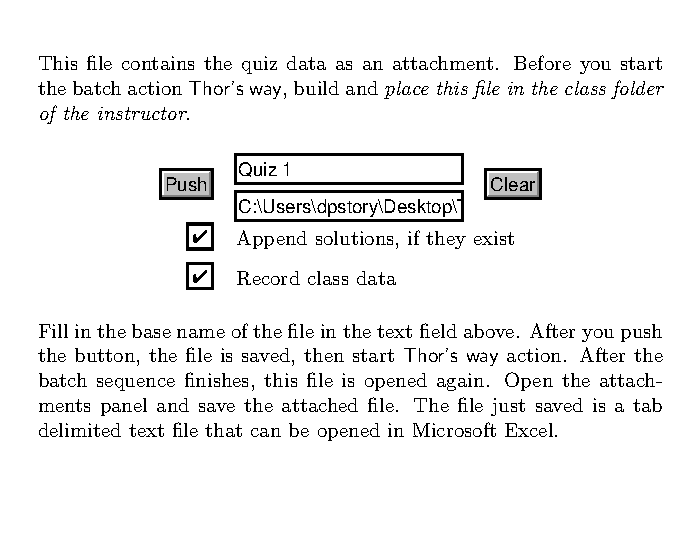
\includegraphics[width=.67\linewidth]{graphics/container}}\\
\caption{\texttt{container.pdf}}\label{cap:container}
\end{figure}

\item With the \texttt{container.pdf} file open, in the top most text field,
    enter a name for the quiz. This will be the base name for the
    tab-delimited TXT file that is attached to \texttt{container.pdf}
\item In the bottom most text field, enter the folder (path) where the quiz files
    are to be saved. (These are the ones named \texttt{\cs{filename-g.pdf}})
    The folder path you enter can be a relative to the folder that contains \texttt{container.pdf},
    or it can be a full (absolute) path to the folder. eg,
    \begin{flushleft}\ttfamily
      /c/users/thor/documents/myuni/spr19/algebra/myclass/graded
    \end{flushleft}
    Notice the method of referencing the path, this is the
    device-independent file path reference in the Acrobat JavaScript API Reference manual.
    See the short article at \href{https://acrobatusers.com/tutorials/print/file-paths-acrobat-javascript}{AcrobatUsers.com}
    for more information.\footnote{On \app{Windows}, a \app{Windows} path seems to work as well: \texttt{c:\string\users\string\thor\string\...\string\graded}}
\item \checkBox[\DV{Yes}\V{Yes}\Ff\FfReadOnly]{apslns}{11bp}{11bp}{Yes} \uif{Append solutions, if they exist}\\
    This check box is checked by default. Clear this box if you don't want
    any solutions to the quiz appended. The \uif{Thor's way} action
    sequence appends the solutions or not according to the state of this
    checkbox.
\item \checkBox[\DV{Yes}\V{Yes}\Ff\FfReadOnly]{rcddt}{11bp}{11bp}{Yes}
    \uif{Record class data}\\
    This check box is checked by default. If you don't want to record the
    class data, clear this check box. Normally, this box is always checked;
    however, if you run \uif{Thor's way} with \uif{Append solutions, if
    they exist} cleared and at a later time you want to append the
    solutions, run \uif{Thor's way} again on the same set of quizzes with
    \uif{Record class data} cleared. The quiz data file attached to the
    \texttt{container.pdf} will be preserved.
\item Now press the button labeled \textsf{Push}. The information of the
    text fields are saved as global JavaScript variables that can be
    accessed by the batch sequence. When you press \textsf{Push}, the file
    \texttt{container.pdf} closes, don't worry.
\end{enumerate}

\newtopic\noindent\textbf{Action phase}\vspace{-6pt}\relax
\begin{enumerate}\setcounter{enumi}{4}
  \item Open the \textsf{Action Wizard} and choose \FmtMP{{Action: }\textsf{Thor's
    way}}\textsf{Thor's way} from
      the list of actions.

\begin{figure}[tbh]\centering\setlength\fboxsep{0pt}
\includegraphics[width=.33\linewidth]{graphics/action-down-arrow}\\
\caption{\textsf{Select files to be processed}}\label{cap:ada}
\end{figure}

  \item \textbf{Select files to be processed.} Click on the down arrow
      control, as indicated in Figure~\ref{cap:ada}. Choose the \textsf{Add
      Folders...} control if your quizzes are in a folder structure,
      \app{Acrobat} should find all PDFs in the folder (including
      subfolders) and list them. Choose the \textsf{Add Files...} controls
      if the quizzes are all in the same folder and you can select them
      all.

\begin{figure}[tbh]\centering\setlength\fboxsep{0pt}
\includegraphics[width=.67\linewidth]{graphics/ManageFiles}\\
\caption{\textsf{ManageFiles dialog box}}\label{cap:fmd}
\end{figure}

  \item \textbf{Select \texttt{terminate-batch.pdf}.} With the \textsf{Add
      Files...}\  control, select the package file \texttt{terminate-batch.pdf}, which resides
      in the same folder as \texttt{control.pdf}. This file must be last in
      the list of files to be processed; if necessary, press the down arrow
      control and select \textsf{Manage Files} (see Figure~\ref{cap:ada}).
      The \textsf{Manage Files} dialog box, Figure~\ref{cap:fmd}, lists all
      the files to be processed. Using the down arrow control in the right,
      move the \texttt{terminate-batch.pdf} to it is last in the list.

\item Keeping your fingers crossed and press the \textsf{Start} control. Each
    of the quizzes is brought into the \app{Acrobat} window, form field
    information is extracted, frozen, saved, and closed.

\item When the \texttt{terminate-batch.pdf} is reached (bottom of the
    list), no extracting or freezing occurs, but what happens is the
    \texttt{control.pdf} document is opened once again.

\begin{figure}[tbh]\centering\setlength\fboxsep{0pt}
\includegraphics[width=.67\linewidth]{graphics/quiz-results}\\
\caption{\textsf{Results displayed}}\label{cap:qr}
\end{figure}

\item Look at the \textsf{Attachments} panel, using the user-interface,
    save the attachment to where you want it. Figure~\ref{cap:qr} shows the
    results of a test run of \textsf{Thor's way}. The produced TXT file is
    a tab-delimited file that can be opened in \textsf{Microsoft Excel}.
    These saved quiz results can be merged, no doubt, into a parent
    \textsf{Excel} spreadsheet.

\end{enumerate}

\subsection{The \tops{\protect\opt{usebatch}}{usebatch} option: multiple renditions source}\label{ss:mr}

The demonstration files for this section are \texttt{thexr.tex} and \texttt{thexrt.tex}.

\newtopic\noindent
In this section we discuss techniques for introducing multiple renditions of
a quiz into the workflow. To be fair the student, the renditions should be roughly equivalent or the students will cry
``foul!'' We don't want that to happen, we have enough troubles.

\subsubsection{Preamble}

Same preamble as previously described, including the use of \cs{sadQuizzes}.

\subsubsection{The body of the document}

Following the \cs{DeclareQuiz} command, declare one or more quiz body names using
the \cs{declareQuizBody} command. Each quiz body declaration has a corresponding quiz
body environment that contains a quiz. A rough outline is seen below.

\begin{Verbatim}[xleftmargin=\amtIndent,commandchars=!()]
%!textsf( declare the name of this quiz)
\DeclareQuiz{!ameta(quiz-name)}

%!textsf( declare the names of the renditions)
\declareQuizBody{!ameta(qb-name!SUB1)}
...
\declareQuizBody{!ameta(qb-name!SUB(k))}

%!textsf( each rendition is a complete quiz within its own environment)
%!textsf( call these environments ``quiz body'' environments)
\begin{!ameta(qb-name!SUB1)}
  !ameta(quiz-rendition!SUB1)
\begin{!ameta(qb-name!SUB1)}
...
\begin{!ameta(qb-name!SUB(k))}
  !ameta(quiz-rendition!SUB(k))
\begin{!ameta(qb-name!SUB(k))}
\end{Verbatim}
Actually, there may be only one rendition ($k=1$), but there is randomness built into
the single rendition to produce a different, yet equivalent, version of the quiz.

The \env{\ameta{qb-name}} environments are verbatim environments that write their contents
to a CUT file, which are later input back into the document.

\newtopic\noindent Following the \env{\ameta{qb-name}} environments comes the final step,
we input these back into the document.
\begin{Verbatim}[xleftmargin=\amtIndent,commandchars=!()]
\InputQuizBody{!ameta(qb-name!SUB1)}
...
\InputQuizBody{!ameta(qb-name!SUB(k))}
\end{Verbatim}
You can input some or all of the declared quiz bodies, and the quiz bodies may be input several
times, especially useful if a quiz body has a degree of randomness built into it.

When you \cs{DeclareQuizBody}, there is an associated version (or rendition)
number in the form of the text macro \cs{QzVer}\FmtMP{\cs{QzVer}}, that
expands to a number (1, 2, 3, and so on). This number can be incorporated
into various section titles, such as in the \cs{sqslsectitle},
\cs{thQzHeader}, and \cs{thQzHeaderCS} commands, for example. Refer to
\texttt{examples/misc/thexrt.tex} for illustrations.

\subsubsection{The \tops{\protect\cs}{\textbackslash}{sadQuizzes} command (revisited)}

When you compile a multi-rendition file, and bring the resulting PDF into a
PDF viewer, you'll see you have $n$-quizzes contained in the document, where
$n$ is the number of \cs{InputQuizBody} commands used. Here is a brief
description of the action of \cs{sadQuizzes} in a multi-rendition document.
\begin{itemize}
  \item If solution pages are present, these pages are extracted from the
      parent document, saved to the instructor's folder, and then
      deleted from the parent document.
  \item If there are cover pages, these are removed and saved to the
      instructor's folder.
  \item As the script goes through the list of students, it extracts one of
      the $n$ quizzes in the parent document and populates it with the name
      data.
  \item If there are cover pages for this quiz set, the cover pages are
      retrieved from the instructor's folder and inserted onto the front of
      the quiz.
  \item The extraction of a subset of pages preserves the document JavaScript,
      but some elements vital to the whole workflow are lost. The script
      restore these lost elements.
  \item It saves each (customized) quiz to the appropriate student folder
      with the file name \cs{jobname-\ameta{first}\_\ameta{last}.pdf}
  \item It saves a copy of the (customized) quiz to the instructor's
      designated folder.
\end{itemize}
What you should get is several versions assigned to the class members:
\begin{itemize}
  \item class member 1 gets the first rendition
  \item class member 2 gets the second rendition
  \item[]...
  \item class member $n$ gets the $n^{\text{th}}$ rendition, where $n = \text{number of \cs{InputQuizBody}}$ statements
  \item class member $n+1$ gets the first rendition
  \item[]...
\end{itemize}
When the parent document is opened in \app{Acrobat}, \cs{sadQuizzes}
executes creates and distributes the quizzes to the instructor's folder and
to the student's individual folder. It's just that simple.

\paragraph*{Student's experience.} Same as their earlier experience, hopefully, this time around it will
be a better experience, better results, happier student, we can only hope.

\paragraph*{Instructor's experience.} Same as above, except {\heshe} has different quizzes to evaluate within
a class. Poor instructor. After {\heshe*} has finished marking the quizzes,
{\heshe*} runs them through \textsf{Thor's way} (\Nameref{sss:TW}), which
leads to happiness for the instructor. The student's score is automatically
recorded\FmtMP{automatically recorded} by the \textsf{Thor's way} action
sequence.

\subsection{Quizzes that specify the \tops{\protect\opt{batchdistr}}{batchdistr} option}\label{ss:bd}

The \opt{batchdistr} option is the same as the \opt{usebatch} option, with
only one difference: After the source file is compiled and opened in
\app{Acrobat}, the newly created quizzes are distributed to the instructor's
folder (as declared by \cs{instrPath}), but \emph{the quizzes are not
distributed to the student folders}. The quizzes are distributed to the
student's folder using batch sequences, to be detailed in subsequent
paragraphs.

\paragraph*{Apply security before distributing quizzes.} The real purpose of
delaying the distribution of the quizzes to the student folders is to place
\emph{password security} on the quiz files. After building the instructor's
copies of the quizzes, the instructor can use the action \textsf{Thor
protects and distributes}. The details of the workflow follows:
\begin{enumerate}
\item \textbf{Build:} Build the source quiz file using the \opt{batchdistr} option.

\item[] When the source file is opened in \app{Acrobat} the first time, the
    custom-named quiz files are saved into the instructor's folder (as
    specified by \cs{instrPath}); no quizzes are deposited in the student
    folders yet.

\item \textbf{Secure and distribute:} With the \app{Acrobat} window empty,
    open the \textsf{Action Wizard} and select the \FmtMP{{Action: }\textsf{Thor
    protects and distributes}}\textsf{Thor protects and distributes} action.
    For the \textsf{Files to be processed}, select the quizzes that have
    just been dropped into the instructor's folder. Perform the action by
    pressing \textsf{Start}.

    Note: To delay the distribution of the quizzes, apply
    \textsf{Thor protects} and later apply \textsf{Thor distributes}.

\item \textbf{Examination period:} Now the students take the quiz, the quiz
    has password security so the student cannot snoop around with the file,
    even if the student has access to \app{Acrobat}.

\item \textbf{Marking period:} Following the exam period, the instructor
    examines each quiz: Press the \textsf{Mark It} button, award any points
    for extended response questions, assign a student grade, and press the
    \textsf{Save \& Close} button.

\item \textbf{Remove security:}\label{item:RS} Press \textsf{Ctrl+K} to
    open the \textsf{Preferences} dialog box. In the left-hand panel,
    select \textsf{Action Wizard}. In the right-hand panel change
    \textsf{Security Method}, using the dropdown menu to \textsf{Password
    Security}. Save your changes by pressing the \textsf{OK} control in the
    lower-right corner.

\item[] With the \app{Acrobat} window empty, open the \textsf{Action
    Wizard} and select the \FmtMP{{Action: }\textsf{Thor removes
    protection}}\textsf{Thor removes protection} action. For the
    \textsf{Files to be processed}, select the quizzes in the student
    folders. Use either \textsf{Add Folder...} or \textsf{Add Files...} to
    select all the quizzes. Perform the action by pressing \textsf{Start}.

\item Press \textsf{Ctrl+K} to open the
    \textsf{Preferences} dialog box. In the left-hand panel, select
    \textsf{Action Wizard}. In the right-hand panel change \textsf{Security
    Method}, using the dropdown menu to \textsf{Do not ask for password}. Save
    your changes by pressing the \textsf{OK} control in the lower-right
    corner.

%Thor allows changes (password) student folders container
\item \textbf{Thor's way:} Now apply the \FmtMP{{Action: }\textsf{Thor's
    way}}\textsf{Thor's way} action, as described in the paragraph
    \textbf{\nameref{para:UTW}} on page~\pageref{para:UTW}.
\end{enumerate}

\section{Bells and whistles}

\subsection{Running Headers}

 The scheme used here assumes no other {\LaTeX} package has been used to take over the running
 headers (and footers). If that is the case, use the values of the commands below to design
 your own.
\bVerb\small\takeMeasure{\string\thQzHeaderCQ\darg{\ameta{text}}}%
\setlength{\eflength}{\widthof{\sffamily(Solutions: \cs{thQuizName})}}%
\edef\x{\the\eflength}%
\setlength{\eflength}{\bxSize}%
\def\1{\rlap{\hskip\eflength\rlap{\hskip\x\relax\quad\cs{def}\cs{th@QzHeaderLQ\darg{\ameta{text}}}}\sffamily(Thor's class)}}
\def\2{\rlap{\hskip\eflength\rlap{\hskip\x\relax\quad\cs{def}\cs{th@QzHeaderCQ\darg{\ameta{text}}}}\sffamily(Quiz \cs{thQuizName})}}
\def\3{\rlap{\hskip\eflength\rlap{\hskip\x\relax\quad\cs{def}\cs{th@QzHeaderCS\darg{\ameta{text}}}}\sffamily(Solutions: \cs{thQuizName})}}
\def\4{\rlap{\hskip\eflength\rlap{\hskip\x\relax\quad\cs{def}\cs{t@hQzHeaderR\darg{\ameta{text}}}}\sffamily(\cs{thepage})}}
\begin{dCmd}[fontsize=\small,commandchars=!()]{\bxSize}
!1\thQzHeaderL{!ameta(text)}
!2\thQzHeaderCQ{!ameta(text)}
!3\thQzHeaderCS{!ameta(text)}
!4\thQzHeaderR{!ameta(text)}
\end{dCmd}
\eVerb These command declarations allow you to set the left, center (for quiz
pages and solution pages), and right running headers. The content of the
parentheses to the right are the default values, which obviously need to be
changed, except, perhaps, for the right header. The declarations in the first column,
define text macros, whose definitions are given in the third column.

The special command \cs{thQuizName} expands to the name of the \ameta{qz-name}, where \ameta{qz-name}
was declare earlier by \cs{DeclareQuiz\darg{\ameta{qz-name}}}. Typically, the choice
for the quiz name very simple, such as \texttt{q1}. You can have a more meaningful
name by declaring \cs{thQzName\darg{\ameta{friendly-qz-name}}}; such a declaration
defines the text macro \cs{thqzname} that expands to \ameta{friendly-qz-name}. The package
initially declares \cs{thQzName\darg{\cs{thQuizName}}}; for example,
\begin{Verbatim}[xleftmargin=\amtIndent]
\thQzHeaderCQ{Pr\"{u}fung: \thqzname}
\thQzHeaderCS{L\"{o}sungen: \thqzname}
\thQzName{Grammatik 1}
\end{Verbatim}
The \cs{rhPgNumsOnly}\FmtMP{\cs{rhPgNumsOnly} discussed} command removes all
running headers, except for the page number in the right header. Expand in
the preamble.

\subsection{Solution pages}

Thor's hammer does support solutions to questions via the usual
\env{solution} environment. When the parent document is built and opened in
\app{Acrobat}, the solution pages are identified, extracted, saved to the
instructor's folder,\footnote{For a parent document that uses basic methods
(no options), the solutions are saved to the current folder of the parent
document.} and deleted from the parent document. As a result, the quiz the
student sees does not contain the solution pages.


\subsection{Cover pages}

While Thor is hammering away on the solution pages, Thor's hammer also
supports the notion cover pages, these are one or more pages appearing in the
front of the parent document (prior to any quizzes). These pages are normally
ignored when the process of building the custom quizzes for the class;
however,  if you declare in the \emph{preamble}\FmtMP{preamble only},
\bVerb\small\takeMeasure{\string\DeclareCoverPage\darg{\ameta{bPg[-ePg]}}}%
%\setlength{\eflength}{\bxSize}%
\begin{dCmd}[fontsize=\small,commandchars=!()]{\bxSize}
\DeclareCoverPage{!ameta(bPg[-ePg])}
\end{dCmd}
\eVerb where \ameta{bPg[-ePg]} are the beginning (\meta{bPg}) and ending
(\meta{ePg}) page numbers; this forms a range of page numbers. As indicated
by the syntax, \cs{ePg} is optional. The values of these page numbers are
0-based\FmtMP{0-based numbering}; that is 0 is the first page of the parent
document, 1 is the second page, and so on. \cs{DeclareCoverPage\darg{0}}
states that page~0 is a cover page, while \cs{DeclareCoverPage\darg{0-1}}
declares the first two pages in the parent document are cover pages. (Page~0
might be a title page, page~1 might be extensive instructions and other
information.) Use your knowledge of {\LaTeX} so that there are no page numbers\FmtMP{no page numbers on cover pages}
on the cover pages.

\subsection{Switches to control program flow}

In this section, we provide switches that give control over the behavior the creation
and function of a quiz.
\bVerb\small\takeMeasure{\string\distrToStudentsOn  \string\distrToStudentsOff}%
%\setlength{\eflength}{\bxSize}%
%\def\1{\rlap{\hskip\eflength D}}
\begin{dCmd}[fontsize=\small,commandchars=!()]{\bxSize}
\autoCopyOn  \autoCopyOff

\instrAutoSaveOn   \instrAutoSaveOff
\instrAutoCloseOn  \instrAutoCloseOff

\stuAutoSaveOn  \stuAutoSaveOff
\stuAutoCloseOn \stuAutoCloseOff

\distrToInstrOn  \distrToInstrOff
\distrToStudentsOn  \distrToStudentsOff
\end{dCmd}
\eVerb The defaults for the above commands are the `On' versions.
\begin{description}
\item[\cmd\autoCopyOn] During document development, you don't want to copy
    the files each time you build and review the document in \app{Acrobat}.
    Set \cs{autoCopyOff} during quiz development, and declare
    \cs{autoCopyOn} when you want to distribute. The default is
    \cs{autoCopyOn}.

\item[\cs{instrAutoSaveOn}] When the instructor presses the freeze quiz
    control, there is an option to automatically save the document or not.
    \cs{instrAutoSaveOn} saves the document; however, if
    \cs{instrAutoSaveOff} is expanded in the preamble, no automatic save is
    performed. The default is \cs{instrAutoSaveOn}.

\item[\cs{instrAutoCloseOn}] When the instructor presses the freeze quiz control, there is an option
    to silently close the document or not. \cs{instrAutoCloseOn} closes the document; however, if
    \cs{instrAutoCloseOff} is expanded in the preamble, no automatic
    closing occurs. The default is \cmd{\instrAutoCloseOn}.

\item[\cs{stuAutoSaveOn}] When expanded in the preamble, a save button will appear
    (created by \cs{stuSaveBtn}) when the \textsf{End Quiz} control is pressed. A
    dialog appears to save the file, the student can choose the file
    location and the file name at that time. When \cs{stuAutoSaveOff} is in
    effect, the save button does not appear, and the student must press the
    save button the on \app{Adobe Reader} toolbar. The default is
    \cs{stuAutoSaveOn}.

\item[\cs{stuAutoSaveOff}] This command is obeyed only if
    \cmd{\stuAutoSaveOn} is in effect. After the student presses the save
    button (\cmd\stuSaveBtn), the document is closed after the student save
    the document. Note that if the student cancels saving the document and
    if the document still needs saving, the document is not closed. The
    default is \cmd\stuAutoCloseOn.

\item[\cs{distrToInstrOff}] Allow the instructor to turn off the
    distribution of the quizzes to himself by using \cs{distrToInstrOff},
    the default is \cs{distrToInstrOn}.

\item[\cmd\distrToStudentsOff] This switch allows the instructor to turn off
    the distribution of the quizzes to the student folders, the default is
    \cs{distrToStudentsOn}. (Note: The \opt{batchdistr} option expands
    \cs{distrToStudentsOff}.

\end{description}
Except for \cs{autoCopyOn} and \cs{autoCopyOff}, there is normally no reason
to change these switches from their defaults. They are here to provide
additional control.

\subsection{Language localization}\label{s:lang}

There are a number of language dependent phrases that appear in the
document, these have conveniently been gathered into the file
\texttt{thorshammer.cfg}. If found on the {\LaTeX} search path, it is
automatically loaded, unless the \opt{nocfg} option is in force. This file
can be localized to your own language, hopefully no umlauts needed.


\subsection{System scripts}\label{s:sysscrpts}

In the course of developing this package, several
\uif{Powershell} system scripts were written to illustrate the
workflow to ourselves. During the long development of this
package, the scripts were folded into a single \uif{Powershell}
script file \texttt{thmclass.ps1}. The use of
\texttt{thmclass.ps1} is described in the file
\texttt{thmclass.pdf}, found in the \texttt{docs} folder.

\begin{comment}
\newtopic\noindent The scripts are assume the folder structure of mighty Thor himself
is used. The scripts use three variables that need to be modified:
\texttt{\$instrName} (\texttt{instrName}), \texttt{\$instrDest}
(\texttt{instrDest}), and \texttt{\$startLocation} (\texttt{startLocation}).
For PowerShell, variables begin with a dollar sign, where is in bash shell
they do not.
\begin{itemize}
   \item \textbf{Windows PowerShell scripts}
   \begin{itemize}
      \item \texttt{getquizzes.ps1}\\ \emph{Copies} every PDF file residing in a folder
      with name \texttt{\$instrName} to the folder defined
      by the path \texttt{\$instrDest}.
      \item \texttt{rmquizzes.ps1}\\ \emph{Removes} (deletes) every PDF file residing in a folder
      with name \texttt{\$instrName}.
      \item \texttt{mvquizzes.ps1}\\ \emph{Moves} every PDF file residing in a folder
      with name \texttt{\$instrName} to the folder defined
      by the path \texttt{\$instrDest}.
   \end{itemize}
\goodbreak
   \item \textbf{Linux bash scripts}
   \begin{itemize}
      \item \texttt{getquizzes.sh}\\\emph{Copies} every PDF file residing in a folder
      with name \texttt{instrName} to the folder defined
      by the path \texttt{instrDest}
      \item \texttt{rmquizzes.sh}\\ \emph{Removes} (deletes) every PDF file residing in a folder
      with name \texttt{instrName}.
      \item \texttt{mvquizzes.sh} \emph{Moves} every PDF file residing in a folder
      with name \texttt{instrName} to the folder defined
      by the path \texttt{instrDest}.
   \end{itemize}
\end{itemize}
Having each quiz in an folder with the instructor's name (\texttt{\_Thor}, or
some other unique name) allows the scripts to find the quiz PDFs, \emph{and no
others}.

\paragraph*{Executing these scripts.} To begin with, I'm no expert. \verb~:-{)~
\begin{itemize}
    \item \textbf{Windows PowerShell scripts.} You must grant the
        permissions for the scripts to executed: open PowerShell (run as
        administrator)1, paste \texttt{Set-ExecutionPolicy RemoteSigned} at
        the prompt and execute this line.
    \item[] The easiest way of working with PowerShell is through the Windows
        PowerShell ISE app. Press the Search icon in the lower left corner of
        windows and type in PowerShell and amongst the matches presented is
        Windows PowerShell ISE. To executed one of the scripts, use the
        File menu to open \texttt{getquizzes.ps1}, for example. There you can edit
        and save the script in the editor provided. To run the script, press the Run Script (F5)
        on the toolbar.
    \item \textbf{Linux bash scripts} On Linux there are permissions to be granted as well, I refer
    the interested reader to \href{https://ryanstutorials.net/bash-scripting-tutorial/bash-script.php}{this web page}.\footnote
    {\url{https://ryanstutorials.net/bash-scripting-tutorial/bash-script.php}} This web page is just one of many
    found by a Google search.
\end{itemize}
\end{comment}

\section{List of sample files}

The sample files are found in the \texttt{example} folder. Fundamentally,
there are only six demonstration files, but these are replicated several times
and distributed over several times in sub-folders of the main \texttt{examples} folder.
The sample files, listed in increasing complexity, and their brief descriptions follow:
\begin{description}
    \item[\texttt{thexb.tex}] uses no option and represents the basic
        methods described in Section~\ref{ss:BMs}.
    \item[\texttt{theuc.tex}] uses the \opt{useclass} option, as described
        in Section~\ref{ss:uc}.
    \item[\texttt{thexub.tex}] uses the \opt{usebatch} option, as described
        in Section~\ref{ss:ub}. The instructor can use \textsf{Thor's way}
        action sequence on these quizzes to automatically record the
        student scores.
    \item[\texttt{thexbd.tex}]  uses the \opt{batchdistr} option, as described
        in Section~\ref{ss:bd}. For this file, distribution of the student
        quizzes is delayed. It is expected to apply some security first.
    \item[\texttt{ther.tex}] uses the \opt{usebatch} option with the
        \opt{allowrandomize} option for \pkg{exerquiz}. As a results,
        certain MC and MS choices are randomized. The \env{quizbody}
        environment encloses the body of the quiz and input back into the
        document twice. As a result, we obtain two versions of the same
        quiz, with two randomized order for MC and MS choices.
    \item[\texttt{theexrt.tex}] uses the \opt{usebatch} option with the
        \opt{allowrandomize} option for \pkg{exerquiz} and uses the
        \pkg{ran\_toks} package as well. The \pkg{ran\_toks} package is
        used to randomize the order of the questions, in addition to the
        randomization of the choices of \texttt{thexr.tex}. The
        \env{quizbody} environment is used twice on two distinct set of
        quiz questions, and input back in several times. The results are
        three ``renditions'' of two distinct quizzes, the order of the
        questions and choices are randomized.
\end{description}
The above files may appear in the following folders.
\begin{description}
   \item [\texttt{nosolns} folder:] This is the original collection of demonstration files,
       all having no solutions associated with any of the questions. (The
       simplest case.)
  \item [\texttt{wthsolns} folder:] The same six demo files, but with selected solutions to
      the questions. The \texttt{thexb.tex} demonstrates how to set of the
      document with a screen design (\opt{designi}). It also uses the
      \pkg{spdef} package (provided) to format the document with or without
      a design option of \pkg{web}. Some of the files use running headers.
  \item[\texttt{cfg} folder:] There are several files in this folder, each
      using the \opt{usebatch} option. They illustrate how to input
      instructor and student data through CFG files, as described in
      section entitled \Nameref{sss:CI}.
  \item[\texttt{misc} folder:] The \texttt{thexrt.tex} file is in this
      folder. The file has been modified several ways.
      \cs{thQuizHeaderLayout} is redefined to hide the \cs{FirstName} and
      \cs{LastName} fields. (Do not delete these two commands, they are
      required, but we can hide them.) Instead of displaying the first and
      last name, the \cs{FullName} command is used on the cover page. The
      \cs{FullName} command gets its value from the values of
      \cs{FirstName} and \cs{LastName}. The changes give the quizzes a
      slightly different look.
  \item[\texttt{target} folder:] The demo files that use the \opt{useclass}
      option, need a target to drop the instructor's copies of the quizzes
      and the student copies of the files. In each of the demo files where
      class information is provided, you need to adjust the paths to taget
      the subfolders of the \texttt{target} folder. The \texttt{target}
      folder may be copied to the desktop, as I did, and target the quiz
      files there.
\end{description}

\section{Summary of action sequences provided}\label{actSeq}

By ``actions sequences'' we mean batch sequences of \app{Acrobat} that
perform a series of tasks. Refer the document
\href{install-action-seq.pdf}{install-action-seq.pdf} for information on
how to install action sequences, found in the \texttt{docs} folder of this
distribution.
\begin{itemize}
  \item\textbf{\textsf{Thor's way} action.} This action is performed on the (student)
      completed and (instructor) marked quizzes. Refer to
      \textbf{\nameref{sss:TW}} on page~\pageref{sss:TW} for more information
      on \textsf{Thor's way}.
      \begin{itemize}
        \item \textbf{Applies to} quizzes compiled with the
            \opt{usebatch} or \opt{batchdistr} option.
        \item\textbf{What it does:} For each quiz, it extracts first
            name, last name, score, total points from the quiz and saves
            them to an attachment of \texttt{container}; it flattens
            the quiz and saves the flattened quiz with a suffix of
            \texttt{"-g"} to the folder designated by the
            \texttt{container} file.
        \item\textbf{Steps to run the \textsf{Thor's way} action}
        \begin{itemize}
          \item Open the file \texttt{container.pdf}
              (\hyperref[cap:container]{Figure~\ref*{cap:container}})
              and fill out the fields provided and press the
              \textsf{Push} button. The file saves the data entered in
              the form fields then closes.
          \item Select the tool \textsf{Action Wizard}, then select
              \textsf{Thor's way}
          \item\textsf{Files to be processed:} Selected the quizzes
              (using the \textsf{Add Folder} and/or \textsf{Add Files}
              controls), then select the special file
              \texttt{terminate-batch.pdf}. This latter file \emph{must
              be the last file to be processed}.
          \item Start the batch by pressing the \textsf{Start} control
        \end{itemize}
      \end{itemize}
      \item[] After the action is finished, the \texttt{control} document
          should be in the \app{Acrobat} window. Check the console window
          to see if there are any errors. The attachment to this file
          contains the quiz results, save and do with them what you will,
          perhaps merging them into a larger spreadsheet.
  \item \textbf{\textsf{Thor protects} action.}\FmtMP{Secret password is \texttt{"acrotex"}} Applies to a collection of
      newly created quizzes that specify the \opt{batchdistr} option.
      Running this action places security on the quizzes so the student's
      cannot view the answers even if they are using \app{Acrobat}.
  \item \textbf{\textsf{Thor distributes} action.} A general purpose action
      that returns quizzes from the instructor's folder (or subfolder) to their
      respective student folders. There are two situations where you would apply
      this action:
      \begin{itemize}
        \item The \textsf{Thor's way} action drops the completed and
            marked quizzes (with suffix \texttt{"-g"}) into the folder
            designated in the \texttt{container} file. This action copies
            them back into the student folders.
        \item For a quiz this is compiled with the \opt{batchdistr}, the
            distribution of the quizzes is delayed (possibly to place
            security restrictions on them using the \textsf{Thor
            protects} action). At the time where you want to deploy the
            quizzes to the students folders, you can use \textsf{Thor
            distributes} to accomplish that task.
      \end{itemize}
  \item \textbf{\textsf{Thor protects and distributes} action.}\FmtMP{Secret password is \texttt{"acrotex"}}  Applies to
      a collection of newly created quizzes that specify the
      \opt{batchdistr} option. Refer to
      \hyperref[ss:bd]{Section~\ref{ss:bd}} for more details. The action is
      to apply security to the quizzes and then to distribute them to the
      student folders. This is a combination of \textsf{Thor protects} and
      \textsf{Thor distributes}.

\goodbreak
      \item[]\textbf{Steps to run the \textsf{Thor protects and distributes} action}
      \begin{itemize}
        \item Select the tool \textsf{Action Wizard}, then select
            \textsf{Thor protects and distributes}
        \item\textsf{Files to be processed:} Selected the quizzes
            (using the \textsf{Add Folder} and/or \textsf{Add Files}
            controls). These are undistributed quizzes and should
            reside in the instructor's folder.
        \item Start the batch by pressing the \textsf{Start} control.
      \end{itemize}
      \item[] After this action is completed, copies of the secured files should
        now be in the student folders.
  \item \textbf{\textsf{Thor removes protection} action.} This action is a
      natural continuation of \textsf{Thor protects and distributes}. It
      removes the security previously placed on the quizzes. This is needed
      to flatten the quizzes later in the work flow. The whole workflow is
      described in \hyperref[ss:bd]{Section~\ref{ss:bd}}. In particular,
      see \hyperref[item:RS]{item~\ref*{item:RS}} titled \textbf{Remove Security}.
      After removing security, we continue with the \textsf{Thor's way} action.
\end{itemize}
\textbf{A Note on Password Protection.} The default password for the two
action sequences is \texttt{"acrotex"}. This can be changed for your system
by editing the two sequences from within the \app{Acrobat} user interface and
changing the password there.

\section{Further discussion of Basic Methods}

The essential difference between these two methods is how the quiz files are
named:
\begin{itemize}
  \item For basic methods, when multiple quiz files are produced, the
      naming convention is \cs{jobname-1.pdf}, \cs{jobname-2.pdf}, and so
      on. When only a single quiz file is created, it is named
      \cs{jobname.pdf}.
  \item For class methods, the quizzes are named as
      \cs{jobname-\ameta{first\SUB1}\_\ameta{last\SUB1}.pdf},
      \cs{jobname-\ameta{first\SUB2}\_\ameta{last\SUB2}.pdf}, and so on.
\end{itemize}
Class methods have three options \opt{useclass}, \opt{usebatch}, and \opt{batchdistr}.
It is the \opt{useclass} that distinguishes basic and class methods.

%\subsection{Basic Methods}
\newtopic\noindent
The following are the scenarios for basic methods:
\begin{itemize}
  \item None of the \textbf{\nameref{para:OCs}} listed on
      page~\pageref{para:OCs} are specified in the preamble. A single quiz
      is produced \emph{for each rendition} in the source file. By default flattening is off, so
      returned quizzes can be run through \textsf{Thor's way} action
      sequence. The source file can be compiled with \cs{flattenOff}, in
      which case manual recording of the grades is needed.
      \begin{itemize}
      \item Files are created in the source file folder.
      \item It is up to the instructor to deliver these quizzes to the
          class.
      \item You can place security on the files using the \textsf{Thor protects} action sequence.
      \end{itemize}
  \item \cs{enumQuizzes\darg{\ameta{num}}}: \ameta{num} copies of the file
      is created (with rendition variations if they exist). All files are
      dropped into the source file folder. Returned files can be run
      through \textsf{Thor's way} to record results, unless \cs{flattenOff}
      is specified in the preamble.
      \begin{itemize}
      \item Analogous to the \opt{usebatch} option.
      \item Files are created in the source file folder.
      \item It is up to the instructor to deliver these quizzes to the
          class.
      \item You can place security on the files using the \textsf{Thor
          protects} action sequence. Quizzes are delivered manually. When
          the returned quizzes are to be marked, use \textsf{Thor removes
          protection} followed by the instructor markup step, followed by
          \textsf{Thor's way} to record the quizzes. This roughly models
          \textsf{batchdistr}, but without the distribution part.
      \end{itemize}
  \item \cs{enumQuizzes\darg{\ameta{num}}} and
        \cs{instrPath\darg{\ameta{path}}} are specified: \ameta{num} copies of the file
      is created (with rendition variations if they exist).  Returned files can be run
      through \textsf{Thor's way} to record results, unless \cs{flattenOff}
      is specified in the preamble.
      \begin{itemize}
      \item Analogous to the \opt{usebatch} option.
      \item All files are dropped into the folder determined by
          \cs{instrPath}.
      \item It is up to the instructor to deliver these quizzes to the
          class.
      \item You can place security on the files using the \textsf{Thor protects} action sequence.
      \end{itemize}

  \item \cs{instrPath\darg{\ameta{path}}},
      \cs{classPath\darg{\ameta{path}}}, and
      \cs{distrQuizzes\darg{\ameta{args}}}: \ameta{num} copies of the file
      is created (with rendition variations if they exist), where
      \ameta{num} is the number of folders listed in the argument of
      \cs{distrQuizzes}.  Returned files can be run through \textsf{Thor's
      way} to record results, unless \cs{flattenOff} is specified in the
      preamble.
      \begin{itemize}
      \item This combination of command best model the \opt{usebatch} option.
      \item A copy of all quizzes are dropped into the folder determined by
          \cs{instrPath}.
      \item A copy of all quizzes are dropped into the student folders determined by
          \cs{classPath}/\cs{distrQuizzes}.
      \item Specifying \cs{distrToStudentsOff} in the preamble, you can
          the place security on the files using the \textsf{Thor protects
          and distributes} action sequence, which places the security on
          the quizzes and distributes them to the student folders. This
          would model the \opt{batchdistr}
      \end{itemize}

  \item \cs{classPath\darg{\ameta{path}}}, and
      \cs{distrQuizzes\darg{\ameta{args}}}: Same as the previous bullet point above.
      \begin{itemize}
      \item This combination of command best model the \opt{usebatch} option.
      \item A copy of all quizzes are dropped into the source folder,
          since no \cs{instrPath} is specified.
      \item A copy of all quizzes are dropped into the student folders determined by
          \cs{classPath}/\cs{distrQuizzes}.
      \item Specifying \cs{distrToStudentsOff} in the preamble, you can
          the place security on the files using the \textsf{Thor protects
          and distributes} action sequence, which places the security on
          the quizzes and distributes them to the student folders. This
          would model the \opt{batchdistr}.
      \end{itemize}


\end{itemize}


\section{A final note on Thor's workflow}

There are two computer drives involved in this workflow: (1) a drive on the
instructor's work computer designated as ID (instructor's drive); and (2) a
system drive that students have access to, designated as SD (system drive).
\begin{enumerate}
\item (ID) The development of the quiz occurs on ID, {\heshe} builds the
    quizzes (perhaps individualized to the names of the students) and saves
    them to the student folders on ID, copies are dumped into the
    instructor's folder on ID.
\item (ID $\mapsto$ SD) The system scripts copy the student folders on ID to
    SD, preserving folder structure.
\item (SD) The class takes the quiz during the quiz period.
\item (SD $\mapsto$ ID) After the quiz period, system scripts copy the
    completed quizzes from the SD student folders to the ID student
    folders, and deletes the quizzes from SD.
\item (ID) The instructor grades each quiz, awarding points for the
    extended response questions. Graded quizzes are flattened and marked
    with a suffix `-g'.
\item (ID $\mapsto$ SD) The system scripts returns the graded quizzes to
    the student folders on SD, where are met with great rejoicing or
    gnashing of teeth.
\end{enumerate}

\section{The \tops{\protect\opt{ordinary}}{ordinary} option}\label{ordinary}

This option was prompted by an \pkg{exerquiz} user who had a unique problem:
He wanted to put password protection (PIN security) on the \uif{Correct}
button of an \pkg{exerquiz} quiz. He wanted to distribute quizzes to his
students. The students would take the quiz, and, on pressing the \uif{End
Quiz} button, would get their score, but the \uif{Correct} button would be
denied to them through a password mechanism.

Solving this problem necessitated some of the special features of
\pkg{thorshammer}, without the use of \cs{sadQuizzes}, as well as the creation
of a few new commands.

To see the solution to this problem, go to the
\texttt{examples/orginary-option} folder to find the demo file
\texttt{thqz-p2c.tex}. This file uses the
\pkg{\href{https://ctan.org/pkg/eq-pin2corr}{eq-pin2corr}} package.\footnote{\pkg{eq-pin2corr} is
a package capable of placing PIN security (and other security) on an \pkg{exerquiz} quiz, apart from the
use of the \pkg{thorshammer} package.}
Additional discussion of the techniques and special ``transition'' commands
is found in the demo document.


\section{My retirement}

Now, I simply must get back to it. \dps

\end{document}

The only user command is \cs{xbmksetup}:
\bVerb\def\1{\qquad}\takeMeasure{\1docbundle=\darg{\ameta{doc\SUB1},\ameta{doc\SUB2},...,\ameta{doc\SUB{n}}},}%
\begin{dCmd}[commandchars=!()]{\bxSize}
\xbmksetup{%
!1docbundle={!ameta(doc!SUB1),!ameta(doc!SUB2),...,!ameta(doc!SUB(n))},
!1colors={int=!ameta(color),ext=!ameta(color)},
!1styles={intbf,extbf,intit,extit}
}
\end{dCmd}
\eVerb

% This code saves a copy of the PDF with the name of each member of the class
% appended. If you have a network drive, you can copy each PDF to their respective
% folders in the connected drive. Here, drive Z: is connected to my PC, drive Z: is
% actually, the C: drive on my other laptop, which is connected to my PC.
% See if this works for you.
%
